\section{Coordinated effects: the MillerCoors joint venture}\label{sec:11-millercoors}

The merger analysis of \cref{sec:11-upp,sec:11-simulation} holds the mode of competition fixed. The merged firm
internalizes the competition among its own products, and every firm continues to set prices as a static
Bertrand-Nash player. Antitrust agencies worry about a second channel as well. The introduction to this chapter
distinguished the two channels informally, and we now state the distinction precisely.

\begin{definition}[Unilateral and coordinated effects]\label{def:11-coordinated}
A merger has \emph{unilateral effects} when it changes prices because the merged firm internalizes the competition
among the products it now owns. All firms keep playing the same static Nash equilibrium. A merger has
\emph{coordinated effects} when it also changes conduct, so that the merged firm and its remaining rivals compete
less aggressively with one another than static Nash pricing implies.
\end{definition}

\citet[p.~238]{AskerNocke2021} make the definition operational. A merger has coordinated effects when it leads to
prices that differ from those of a static Nash equilibrium. Any model of such effects therefore needs a continuation
value, which usually takes the defect-and-punish form of the collusion models of \cref{ch:collusion-theory}. The
idea is old. In the words of \citet{Stigler1964}, ``[c]ollusion of firms can take many forms, of which the most
comprehensive is outright merger''.
Section 7.2 of the 2010 Horizontal Merger
Guidelines discusses the market conditions that facilitate collusion \citep{USDOJFTC2010}, as \citet[p.~203,
n.~67]{AskerNocke2021} note. Merger challenges invoke coordinated effects often. Richard Gilbert and Hillary Greene
counted the merger complaints filed by the DOJ and the FTC between 1990 and 2014. In their count, as cited by
\citet{MillerWeinberg2017}, 60 percent alleged coordinated effects of some form \citep[p.~238,
n.~154]{AskerNocke2021}. Economists, by contrast, have concentrated on unilateral effects since the
1980s. Asker and Nocke attribute the focus to the analytical clarity of unilateral effects and to the lack of clear
empirical examples that link mergers to more coordination (pp.~238--239). \Cref{sec:11-ce-theory} sets out what the
theory says, and the rest of the section studies one of the few empirical examples.

\citet{MillerWeinberg2017} provide one of the first structural estimates of the coordinated effects of a consummated
merger.
They study the 2008 joint venture that combined the US brewing operations of SABMiller and Molson Coors into a new
firm, MillerCoors. Their method nests static Bertrand-Nash pricing inside a model in which the merged firm and its
largest rival put a weight $\kappa$ on each other's profits. It then estimates $\kappa$ from the post-merger prices.
This section follows the paper from its question to its contribution. It derives every estimating equation, proves
the properties of the estimator that the paper relies on, and reproduces Tables IV, V, VI and X.\footnote{Page
numbers in this section refer to the journal article. We change three pieces of the paper's notation to keep the
book consistent. The paper's nesting parameter $\rho$ is our $\sigma$ (in this book $\rho$ is pass-through). Its
product, period and region effects $\sigma_j$, $\tau_t$ and $\mu_r$ are our $\varphi_j$, $\tau_t$ and $\upsilon_r$.
The paper writes utility as $+\alpha p$ with $\alpha < 0$, while we write $-\alpha p$ with $\alpha > 0$. The tables
keep the paper's signs.}

\subsection{The theory of coordinated effects}\label{sec:11-ce-theory}

The theory of coordinated effects comes from the repeated games of \cref{ch:collusion-theory}. The question is
whether a change in market structure makes collusion easier to sustain, in the sense that it lowers the critical
discount factor above which collusion is an equilibrium. We follow \citet[pp.~239--240]{AskerNocke2021}, first in
the symmetric benchmark and then with capacities.

\casehead{Symmetric Bertrand competition}
Let $N$ symmetric firms sell a homogeneous good at constant marginal cost and set prices in every period of an
infinitely repeated game with discount factor $\delta$. Suppose all firms charge the monopoly price $p^m$ and share
the monopoly profit $\pi^m$ equally, and any deviation triggers static Bertrand pricing at marginal cost forever. A
firm that undercuts slightly takes the whole market for one period and earns close to $\pi^m$, and zero thereafter.
Collusion is an equilibrium if and only if
\begin{equation*}
\frac{1}{1 - \delta}\cdot\frac{\pi^m}{N} \ge \pi^m
\quad\Longleftrightarrow\quad
1 \ge N(1 - \delta)
\quad\Longleftrightarrow\quad
\delta \ge \underline\delta_N = 1 - \frac{1}{N} .
\end{equation*}
A merger from $N$ to $N - 1$ firms lowers the critical discount factor from $1 - \frac{1}{N}$ to $1 - \frac{1}{N -
1}$, so collusion becomes sustainable for more discount factors. Under imperfect monitoring, the time the industry
spends in the collusive state also falls with $N$. On this account, mergers facilitate collusion.

The model is special, because neither the deviation profit ($\pi^m$) nor the punishment profit (zero) depends on
$N$. In richer models both can fall with the number of firms. A merger then raises both the gain from cooperating
and the gain from deviating, and its effect on the critical discount factor is ambiguous. Firms also differ, and a
merger does more than remove a competitor, since the merged firm obtains the partners' tangible and intangible
assets.

\casehead{Capacity constraints}
\citet{CompteJennyRey2002} show how asymmetries change the answer. Demand is one unit at any price up to the monopoly
price of one, and zero above it. Firm $i$ has zero marginal cost up to its capacity $k_i$, with $k_1 \le k_2 \le
\dots \le k_N$. Write $\hat k_i = \min\{k_i, 1\}$ for firm $i$'s \emph{effective capacity}, $\hat K = \sum_i\hat k_i$
for the sum of effective capacities, and $K_{-N} = \sum_{i < N}k_i$ for the capacity of all firms but the largest.
Monitoring is perfect, and attention is restricted to equilibria in which each firm keeps the same market share
$\omega_i$ along every continuation path.
A merger of firms $l$ and $m$ combines their capacities into $k_l + k_m$
and creates no efficiencies.

\begin{proposition}[Capacities and collusion, \citealp{CompteJennyRey2002}]\label{prop:11-cjr}
\leavevmode
\begin{enumerate}[label=(\alph*)]
\item If $K_{-N} \ge 1$, perfect collusion at price one is sustainable if and only if
$\delta \ge \underline\delta = \frac{\hat K - 1}{\hat K}$, and the best shares are $\omega_i = \frac{\hat
k_i}{\hat K}$. If $K_{-N} \ge 1$ holds before and after a merger of $l$ and $m$, the merger weakly lowers
$\underline\delta$, and strictly if and only if $k_l + k_m > 1$.
\item If $K_{-N} < 1$, the largest firm's incentive constraint binds under the best allocation of shares, and
$\underline\delta = \frac{\hat k_N}{\hat K}$. A merger involving the largest firm raises $\underline\delta$. A
merger that does not involve the largest firm and does not create a new largest firm leaves it unchanged.
\end{enumerate}
\end{proposition}

\begin{proof}[Proof of part (a)]
Every firm's rivals together have capacity at least $K_{-N} \ge 1$, so they can serve the whole market. In the
static game the price is therefore zero and every firm earns zero, which is the harshest possible punishment. Under
collusion firm $i$ earns $\omega_i$ per period. Its best deviation prices just below one and sells $\hat k_i$, and it
earns zero afterward. It does not deviate if and only if
\begin{equation*}
\frac{\omega_i}{1 - \delta} \ge \hat k_i
\quad\Longleftrightarrow\quad
\delta \ge 1 - \frac{\omega_i}{\hat k_i} .
\end{equation*}
Collusion is sustainable if and only if $\delta \ge \max_i\big(1 - \frac{\omega_i}{\hat k_i}\big)$, so the best
shares maximize $\min_i\frac{\omega_i}{\hat k_i}$ subject to $\sum_i\omega_i = 1$. Because $\sum_i\hat
k_i\cdot\frac{\omega_i}{\hat k_i} = 1$, a weighted average of the ratios $\frac{\omega_i}{\hat k_i}$ with weights
$\frac{\hat k_i}{\hat K}$ equals $\frac{1}{\hat K}$. Their minimum is therefore at most $\frac{1}{\hat K}$, with
equality when every ratio equals $\frac{1}{\hat K}$. Hence $\underline\delta = 1 - \frac{1}{\hat K}$. A merger
replaces $\hat k_l + \hat k_m$ by $\min\{k_l + k_m, 1\}$, which is never larger and is strictly smaller if and only if
$k_l + k_m > 1$. A smaller $\hat K$ lowers $1 - \frac{1}{\hat K}$.
\end{proof}

Part (b) requires optimal punishments with two phases, a low price in the first period of the punishment and a high
price afterward. Static Nash pricing no longer holds the firms to their minmax payoffs
\citep[p.~240, n.~156]{AskerNocke2021}. We state part (b) without proof. The two parts reverse the symmetric intuition in
different ways. In part (a) a merger helps collusion only by destroying effective capacity. In part (b) a merger
that makes the largest firm larger makes the industry more asymmetric and hurts collusion. With capacities $(0.2,
0.3, 0.4, 1.0)$, for example, $K_{-N} = 0.9$ and $\underline\delta = \frac{1}{1.9} \approx 0.53$. A merger of the
largest firm with the smallest gives $(0.3, 0.4, 1.2)$ and $\underline\delta = \frac{1}{1.7} \approx 0.59$. A merger
of the two smallest gives $(0.4, 0.5, 1.0)$ and leaves $\underline\delta$ at 0.53.

\casehead{What the theory can and cannot say}
In a model with heterogeneous firms, a merger may thus help or hinder collusion, depending on the market and the
merger. Outside very special models the conditions are not well understood, and the theory gives no robust mapping
from a critical discount factor to the probability that collusion occurs \citep[p.~240]{AskerNocke2021}.
\citet{KaplowShapiro2007} put the problem sharply. Supergame theory with patient players predicts collusion for
almost any market structure, so it ``proves too much'' (n.~159). It is not surprising that courts in the last twenty
years have been reluctant to block mergers on coordinated-effects grounds, unless the industry had been cartelized
before. Conversely, a merger in an industry that is already cartelized may do little harm, and its efficiencies may
benefit society. \citet{RollerSteen2006} study a cartel in the Norwegian cement industry between 1955 and 1968. It
allocated market shares by capacity, which led to overinvestment in capacity. The 1968 merger of the industry's two
firms solved the coordination problem and removed the incentive to overinvest. Relative to wasteful collusion, this
merger to monopoly raised welfare, although competition would have raised it more (n.~160). Recent research gives
the concern a firmer empirical basis, and \citet{MillerWeinberg2017} is its leading example (p.~240).

\subsection{The question}\label{sec:11-mc-question}

The economic question is why the prices of the largest domestic beers rose after the joint venture, and whether the
rise reflects a change in how the remaining brewers compete. The joint venture combined the second and third largest
US brewers. A standard merger simulation predicts that the merged firm raises its prices, that rivals raise theirs a
little through strategic complementarity, and that efficiencies push in the other direction. The data show something
the standard model struggles to produce. The price of Bud Light, the flagship of the largest rival, rose by about as
much as the prices of Miller Lite and Coors Light. The prices of the leading imports did not rise.

The question matters for three reasons. First, it tests the maintained assumption of every merger simulation in
\cref{sec:11-simulation}, namely that post-merger conduct is static Nash. Second, it separates three forces that
act on post-merger prices at the same time: unilateral effects, coordinated effects and cost efficiencies. Third,
the US Department of Justice (DOJ) cleared the joint venture on the strength of its expected efficiencies. The
paper can ask whether that decision was right under different welfare standards.

The answer has three parts \citep[pp.~1781 and 1788]{MillerWeinberg2017}. The estimated internalization parameter is
between 0.25 and 0.37 and is significantly different from zero, so post-merger Nash-Bertrand pricing is rejected.
The joint venture produced large marginal-cost savings for MillerCoors, which roughly offset its unilateral effects.
Coordination raised the prices of all three domestic brewers well above their no-merger levels, so consumers lost
while total surplus rose slightly.

\subsection{The industry and the event}\label{sec:11-mc-industry}

The US beer market has many brands but few large brewers. Around the time of the joint venture, five firms
controlled about 80 percent of US retail revenue. Anheuser-Busch InBev (ABI), the owner of Budweiser and Bud Light, was the largest, with
about 35 percent. SABMiller (Miller) and Molson Coors (Coors) were the next two. Grupo Modelo (Corona) and Heineken
together held about 15 percent. Real beer prices fell between 2000 and 2008. \Cref{tab:11-mw-brands} lists the 13
brands in the paper's sample by owner.

\begin{table}[htbp]
\centering
\caption{Brewers and brands in the Miller and Weinberg sample}
\label{tab:11-mw-brands}
\footnotesize
\begin{tabular}{@{}lll@{}}
\toprule
Brewer (after June 2008) & Brands (row number in \cref{tab:11-mw-elast}) & Origin \\
\midrule
ABI & Bud Light (1), Budweiser (2), Michelob (9), Michelob Light (10) & Domestic \\
MillerCoors: Coors brands & Coors (3), Coors Light (4) & Domestic \\
MillerCoors: Miller brands & Miller Genuine Draft (11), Miller High Life (12), Miller Lite (13) & Domestic \\
Modelo & Corona Extra (5), Corona Light (6) & Imported \\
Heineken & Heineken (7), Heineken Light (8) & Imported \\
\bottomrule
\end{tabular}

\smallskip
\begin{minipage}{0.95\linewidth}
\footnotesize Notes: Each brand is sold in 6, 12 and 24 packs, and a product is a brand and package size. Before June
2008 the Miller and Coors brands belonged to separate firms. The brand list is the row list of
\citet[Table V]{MillerWeinberg2017}. Ownership is as described in the text.
\end{minipage}
\end{table}

The joint venture was announced on October 9, 2007 \citep[p.~9]{AshenfelterHoskenWeinberg2015} and consummated in June 2008
\citep[p.~1768]{MillerWeinberg2017}.
It combined the US operations of SABMiller and Molson Coors, with a combined share of about 30 percent. The DOJ
reviewed it as a merger and approved it on June 5, 2008. It found that efficiencies from combining the brewing
operations would outweigh any adverse competitive effect \citep[p.~241, n.~161]{AskerNocke2021}. The savings were in
shipping and distribution. Coors brewed in two locations and Miller in six. Moving Coors production into Miller
plants let the venture brew beer closer to many of its 48 regional markets \citep[pp.~219--220]{AskerNocke2021}. The
same investigation also surfaced documents that pointed to leader-follower pricing in the industry (p.~241).
\citet[p.~1788]{MillerWeinberg2017} consider a scenario with unilateral effects and efficiencies but no
coordination. They describe it as the one ``deemed most likely by the DOJ in its decision to clear the merger.''

Three institutional features matter for what follows. First, US beer is sold through a \emph{three-tier system}:
brewers sell to independent distributors, who sell to retailers. The model of the paper lets brewers sell directly
to consumers and treats the retail sector in a supplemental appendix \citep[p.~1779]{MillerWeinberg2017}. Second,
InBev acquired Anheuser-Busch in November 2008, five months after the joint venture \citep[p.~1784]{MillerWeinberg2017}.
Third, Anheuser-Busch held a large equity stake in Grupo Modelo during the sample period. \Cref{fig:11-beer} records it
as 50.3 percent before ABI bought the rest of Modelo in a \$20.1 billion deal. That acquisition came in 2013, after the
sample period \citep[p.~1767]{MillerWeinberg2017}. The second and third facts reappear in the assessment in
\cref{sec:11-mc-assessment}.

\subsection{Facts and hypotheses}\label{sec:11-mc-facts}

\Cref{fig:11-mwfacts} reproduces the paper's Figure 1. It plots the average log real price of a 12 pack of five
flagship brands from 2001 to 2011, in 2010 dollars. Before the joint venture, Miller Lite, Coors Light and Bud Light
move almost in lockstep and drift down. After June 2008 all three jump by roughly 6 log points and stay at the higher
level through 2011.\footnote{The 6 log point jump is our reading of the figure, from about 2.25--2.27 before June
2008 to about 2.29--2.33 afterwards. \citet[p.~242]{AskerNocke2021}, who reproduce the figure, describe the jump as
an 8 percent increase in the prices of all three brands. The paper itself states an increase of about 8 percent
\citep[p.~1768]{MillerWeinberg2017}, so we report both. The paper notes the brief dip in Miller Lite prices just
after the merger in its footnote 5.} Corona Extra and Heineken keep falling. In the paper's words, the imports ``do not exhibit any
persistent increase and instead continue along a downward trend'' \citep[p.~1769]{MillerWeinberg2017}. The price
gap between domestic beers and imports therefore shrinks.

\begin{figure}[htbp]
\centering
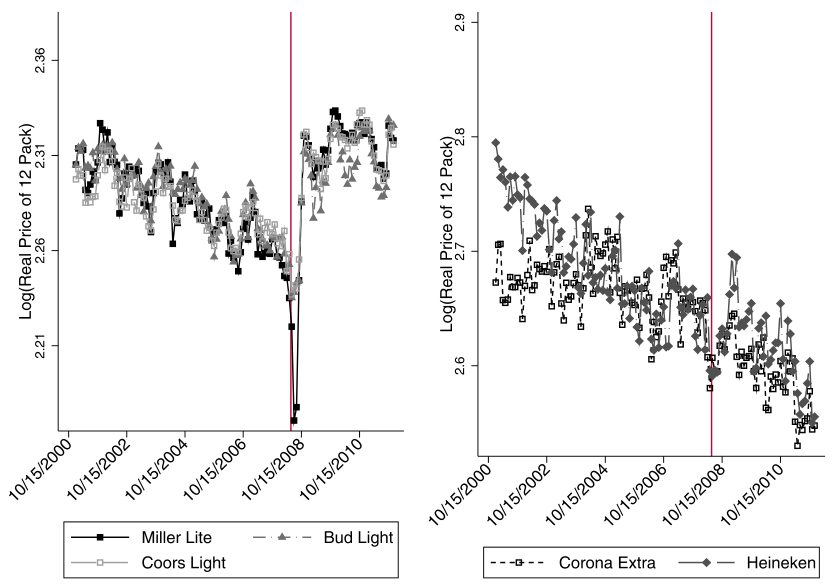
\includegraphics[width=0.92\textwidth]{figures/ch11/mw_fig1_prices.png}
\caption{Average retail prices of flagship 12 packs, 2001--2011. The left panel shows Miller Lite, Bud Light and Coors
Light, and the right panel shows Corona Extra and Heineken. The vertical axis is the natural log of the price in real
2010 dollars, and the vertical line marks the consummation of the joint venture in June 2008. Source: Miller and
Weinberg (2017), Figure 1.}
\label{fig:11-mwfacts}
\end{figure}

\citet[p.~1769]{MillerWeinberg2017} single out two features of the figure. The price of Bud Light rises by roughly
the same amount as the prices of Miller Lite and Coors Light. The prices of the Modelo and Heineken brands do not
rise, at least not persistently. They list four explanations that are consistent with these facts.
\begin{enumerate}[label=(H\arabic*)]
\item ABI and MillerCoors \emph{coordinate} after the merger and compete less aggressively with each other.
\item \emph{Unilateral effects} alone explain the data. Demand could make domestic beer prices strong strategic
complements of one another and weak strategic complements of import prices. Then ABI would follow MillerCoors up even
under Nash pricing, while importers would not.
\item \emph{Institutional practices} explain the data. Retailers might price Bud Light, Miller Lite and Coors Light
equally whatever happens to costs and demand, out of habit or under pressure from brewers.
\item The \emph{Great Recession} explains the data. The recession began at about the time of the merger. Lower incomes
could make domestic beer demand less elastic, for example through down-market substitution from imports.
\end{enumerate}
The paper weighs (H4) with a fact. Sales of the domestic brands fell in both absolute and relative terms during the
recession, which is hard to square with consumers trading down to them \citep[n.~5]{MillerWeinberg2017}.

The test the paper builds follows from (H1) and (H2). If unilateral effects alone explain the data, an estimated
demand system plus Nash pricing should reproduce the post-merger price of Bud Light. If they cannot, a model with
partial internalization of the ABI-MillerCoors pricing externality should fit better. The test therefore requires a
demand system rich enough to give (H2) a fair chance, and a supply model in which Nash pricing is a special case. The
logic is the same as in the conduct-parameter literature of \cref{ch:conduct}. The new element is a change in conduct
at a known date, caused by a known change in market structure.

\subsection{Theory: partial internalization of pricing externalities}\label{sec:11-mc-theory}

We first develop the supply model in general form. Consider one market and drop the region and period indices. There
are $J$ products and $F$ firms, and firm $f$ sells the products in $\mathcal{J}_f$. Market size is $M$, the share of
product $j$ is $s_j(p)$, marginal cost $mc_j$ is constant, and firm $f$'s variable profit is
\begin{equation}\label{eq:11-mc-profit}
  \pi_f(p) = M\sum_{k \in \mathcal{J}_f}(p_k - mc_k)\, s_k(p).
\end{equation}

\begin{assumption}[Partial internalization]\label{ass:11-mc-kappa}
(i) Firm $f$ chooses the prices of its products to maximize
\begin{equation}\label{eq:11-mc-objective}
  V_f(p) = \pi_f(p) + \sum_{g \neq f}\kappa_{fg}\,\pi_g(p),
\end{equation}
taking the prices of other firms as given, with weights $\kappa_{fg} \in [0,1]$ and $\kappa_{fg} = \kappa_{gf}$.
(ii) A Nash equilibrium of the game with payoffs $V_f$ exists and is interior.
\end{assumption}

\Cref{sec:11-simframework} stated the resulting first-order conditions without proof, and the worked example of
\cref{sec:11-logitex} used them. The weight $\kappa_{fg}$ is the fraction of rival $g$'s profit that firm $f$ counts
as its own. With all weights
equal to zero, the model is the multiproduct Bertrand-Nash model of \cref{ch:diffprod}. With $\kappa_{fg} = 1$, firms
$f$ and $g$ maximize their joint profit, exactly as if they had merged. Intermediate weights have two readings. The
first is literal: if firm $f$ owns a share of firm $g$'s equity, its owners gain from $g$'s profit
\citep{OBrienSalop2000}. The second is a reduced form for tacit coordination, which is the reading
\citet[p.~1779]{MillerWeinberg2017} adopt. They call $\kappa$ the ``post-merger internalization of coalition pricing
externalities.''

\begin{proposition}[First-order conditions with partial internalization]\label{prop:11-mc-foc}
Let $\Delta$ be the $J \times J$ matrix with $(j,k)$ element $\frac{\partial s_j}{\partial p_k}$, and let $\Omega(\kappa)$
be the matrix with $(j,k)$ element $\kappa_{f(j)f(k)}$, where $f(j)$ is the owner of product $j$ and $\kappa_{ff} = 1$.
Under \cref{ass:11-mc-kappa} equilibrium prices satisfy
\begin{equation}\label{eq:11-mc-foc}
  s(p) + \big(\Omega(\kappa) \odot \Delta(p)^\top\big)(p - mc) = 0 ,
\end{equation}
and, when the matrix is invertible, the markup vector is
\begin{equation}\label{eq:11-mc-markup}
  p - mc = b(p;\kappa) \equiv -\big[(\Omega(\kappa) \odot \Delta(p))^\top\big]^{-1} s(p).
\end{equation}
\end{proposition}

\begin{proof}
Take $j \in \mathcal{J}_f$. Differentiating \eqref{eq:11-mc-objective} with \eqref{eq:11-mc-profit} gives
\begin{align*}
  \frac{\partial V_f}{\partial p_j}
  &= M\Big[s_j + \sum_{k \in \mathcal{J}_f}(p_k - mc_k)\frac{\partial s_k}{\partial p_j}\Big]
     + \sum_{g \neq f}\kappa_{fg}\, M\sum_{k \in \mathcal{J}_g}(p_k - mc_k)\frac{\partial s_k}{\partial p_j} \\
  &= M\Big[s_j + \sum_{k=1}^{J}\kappa_{f(j)f(k)}\,(p_k - mc_k)\,\Delta_{kj}\Big].
\end{align*}
The second line uses $\kappa_{ff} = 1$ and collects all products into one sum. Setting the derivative to zero and
dividing by $M > 0$ gives $s_j + \sum_k \Omega_{jk}(\Delta^\top)_{jk}(p_k - mc_k) = 0$ for every $j$. Stacking the $J$
equations gives \eqref{eq:11-mc-foc}. Symmetry of the weights makes $\Omega(\kappa)$ symmetric, so
$\Omega \odot \Delta^\top = (\Omega \odot \Delta)^\top$, and solving for $p - mc$ gives \eqref{eq:11-mc-markup}.
\end{proof}

Equation \eqref{eq:11-mc-markup} is the markup formula of \cref{ch:blp} (\cref{eq:08-markup}) with the ownership
matrix replaced by $\Omega(\kappa)$. \citet[eq.~(9)]{MillerWeinberg2017} write it as
$p_t = mc_t - [\Omega_t(\kappa) \circ (\frac{\partial s_t}{\partial p_t})^\top]^{-1}s_t$, which is the same object.
In their application the weight is nonzero only for pairs of ABI and MillerCoors products after the merger. Let
$\mathcal{J}_A$, $\mathcal{J}_M$, $\mathcal{J}_O$ and $\mathcal{J}_H$ be the products of ABI, MillerCoors, Modelo and
Heineken, and write $\mathbf{1}$ for a matrix of ones of the conformable size. Ordering products by firm, the
post-merger matrix is
\begin{equation}\label{eq:11-mc-omega13}
  \Omega^{post}(\kappa) =
  \begin{bmatrix}
    \mathbf{1}_{AA} & \kappa\mathbf{1}_{AM} & 0 & 0 \\
    \kappa\mathbf{1}_{MA} & \mathbf{1}_{MM} & 0 & 0 \\
    0 & 0 & \mathbf{1}_{OO} & 0 \\
    0 & 0 & 0 & \mathbf{1}_{HH}
  \end{bmatrix}.
\end{equation}
Before the merger the Miller and Coors blocks are separate, so $\Omega^{pre}$ is block diagonal with five blocks.
The paper illustrates with a hypothetical region in which ABI, Miller, Coors and Modelo each sell one product
\citep[eq.~(10)]{MillerWeinberg2017}:
\begin{equation}\label{eq:11-mc-omega4}
  \Omega_{t_1^*} =
  \begin{bmatrix} 1 & 0 & 0 & 0 \\ 0 & 1 & 0 & 0 \\ 0 & 0 & 1 & 0 \\ 0 & 0 & 0 & 1 \end{bmatrix},
  \qquad
  \Omega_{t_2^*} =
  \begin{bmatrix} 1 & \kappa & \kappa & 0 \\ \kappa & 1 & 1 & 0 \\ \kappa & 1 & 1 & 0 \\ 0 & 0 & 0 & 1 \end{bmatrix},
\end{equation}
where $t_1^*$ is a pre-merger period and $t_2^*$ a post-merger period. Miller and Coors fully internalize each other
after the merger, ABI and MillerCoors internalize each other with weight $\kappa$, and Modelo prices as a Nash
player. The last feature is a restriction. The paper imposes it for Modelo and Heineken on the basis of qualitative
evidence \citep[p.~1779]{MillerWeinberg2017}.

\begin{remark}[$\kappa$ and the conduct parameter]\label{rem:11-mc-theta}
In a homogeneous-good market with $N$ symmetric firms, constant marginal cost $c$ and inverse demand $P(Q)$, let each
firm maximize $\pi_i + \kappa\sum_{j \neq i}\pi_j$ over its output. The first-order condition is
\begin{equation*}
  P(Q) + q_i P'(Q) - c + \kappa P'(Q)\sum_{j \neq i}q_j = 0 .
\end{equation*}
At a symmetric equilibrium $q_i = \frac{Q}{N}$ and $\sum_{j\neq i}q_j = \frac{(N-1)Q}{N}$, so
\begin{equation*}
  P(Q) - c + \theta\, Q P'(Q) = 0, \qquad \theta = \frac{1}{N} + \kappa\,\frac{N-1}{N}.
\end{equation*}
This is the conduct-parameter form of \cref{ch:conduct}. The weight $\kappa = 0$ gives Cournot ($\theta = \frac{1}{N}$)
and $\kappa = 1$ gives monopoly ($\theta = 1$). The internalization weight is thus a conduct parameter, and the
critique of \citet{Corts1999} applies to it. \Cref{sec:11-mc-assessment} returns to this point.
\end{remark}

The next result says how $\kappa$ changes pricing incentives at pre-merger prices. It extends the upward pricing
pressure (UPP) of \cref{sec:11-upp} to partial internalization. Write $D_{jk} = -\frac{\Delta_{kj}}{\Delta_{jj}}$
for the diversion ratio from $j$ to $k$ and $m_k = p_k - mc_k$ for the margin.

\begin{proposition}[Pricing pressure with partial internalization]\label{prop:11-mc-upp}
Suppose pre-merger prices satisfy \eqref{eq:11-mc-foc} with $\Omega^{pre}$, and evaluate the post-merger objectives at
pre-merger prices and costs. Then the post-merger pricing pressure on each product is:
\begin{align}
  \text{ABI product } j \in \mathcal{J}_A: &\quad UPP_j = \kappa\sum_{k \in \mathcal{J}_M} m_k D_{jk}, \label{eq:11-mc-upp-abi}\\
  \text{Miller product } j: &\quad UPP_j = \sum_{k \in \text{Coors}} m_k D_{jk} + \kappa\sum_{k \in \mathcal{J}_A} m_k D_{jk},
  \label{eq:11-mc-upp-mc}\\
  \text{import } j \in \mathcal{J}_O \cup \mathcal{J}_H: &\quad UPP_j = 0. \notag
\end{align}
The expression for a Coors product exchanges the roles of Miller and Coors in \eqref{eq:11-mc-upp-mc}.
\end{proposition}

\begin{proof}
Take $j \in \mathcal{J}_A$. At pre-merger prices the pre-merger condition holds:
$s_j + \sum_{k \in \mathcal{J}_A} m_k \Delta_{kj} = 0$. The post-merger derivative of $\frac{V_A}{M}$ with respect to
$p_j$ is the same expression plus $\kappa\sum_{k \in \mathcal{J}_M} m_k \Delta_{kj}$. At pre-merger prices it therefore
equals $\kappa\sum_{k\in\mathcal{J}_M} m_k\Delta_{kj}$. Dividing by $-\Delta_{jj} > 0$ converts it into dollars per
unit, as in \cref{sec:11-upp}:
\begin{equation*}
  \frac{\kappa\sum_{k\in\mathcal{J}_M} m_k\Delta_{kj}}{-\Delta_{jj}} = \kappa\sum_{k\in\mathcal{J}_M} m_k D_{jk}.
\end{equation*}
For a Miller product the post-merger objective adds the Coors products with weight one and the ABI products with
weight $\kappa$, and the same steps give \eqref{eq:11-mc-upp-mc}. Import objectives do not change.
\end{proof}

Under Nash pricing ($\kappa = 0$) ABI faces no direct pressure. Its prices rise only through strategic
complementarity, because MillerCoors's higher prices raise the demand for ABI's products. With $\kappa > 0$, ABI
faces pressure equal to $\kappa$ times the pressure it would face if it had merged with MillerCoors. This is the
sense in which coordination makes the largest rival behave like a partial merger partner. Efficiencies enter the
MillerCoors expressions as a credit $E_j mc_j$, exactly as in \cref{prop:11-netupp}.

Coordination also changes how rivals respond to the merged firm's efficiencies. In the Nash model a cost reduction at
MillerCoors lowers MillerCoors's prices, and strategic complementarity then lowers ABI's prices. With $\kappa > 0$
there is a countervailing force. A larger MillerCoors margin raises the value to ABI of the sales it diverts to
MillerCoors, so ABI wants to raise its price. \Cref{fig:11-mwident} shows the result in the logit illustration of
\cref{ex:11-logit}, which is also the example of \citet[p.~1780]{MillerWeinberg2017}. Three symmetric single-product
firms face logit demand with price 1.00, marginal cost 0.70, inside shares of 0.20 and an outside share of 0.40, and
firms 1 and 2 merge. At $\kappa = 0$ the rival price $p_3$ rises with the merged firm's cost $c_M$, with slope 0.061 at
$c_M = 0.6$. At $\kappa = 0.5$ the slope is $-0.148$.\footnote{These slopes and the contours in
\cref{fig:11-mwident} are our computations.} The figure also
previews the identification argument of \cref{sec:11-mc-supply}. The merging-firm price $p_M$ and the rival price
$p_3$ trace two families of curves that cross. An observed pair $(p_M, p_3)$ therefore pins down both the
internalization weight and the efficiency. For example, the pair $(1.09, 1.08)$ reported in the paper's third case
corresponds to $\kappa = 0.53$ and $c_M = 0.68$ in our computation (\cref{rem:11-mw-typo} discusses this case).

\begin{figure}[htbp]
\centering
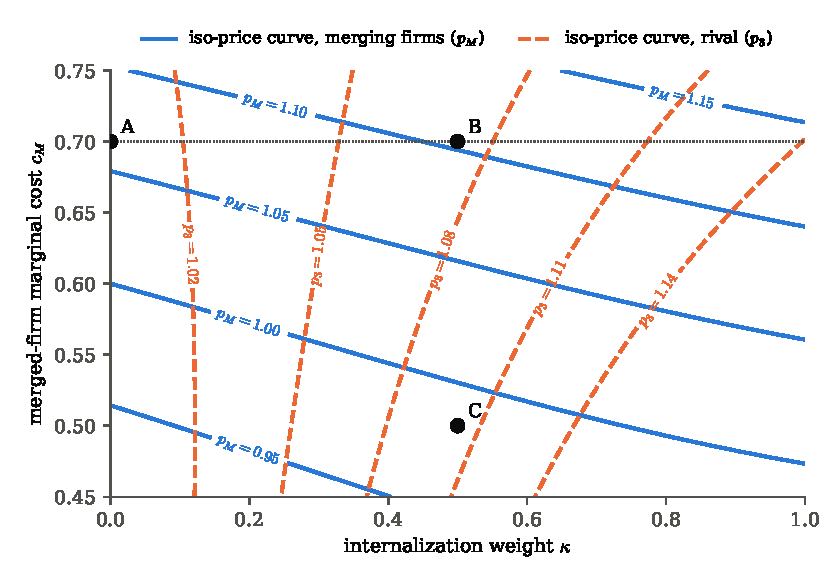
\includegraphics[width=0.82\textwidth]{figures/ch11/mw_identification.pdf}
\caption{Identification of the internalization weight and the efficiency in the logit illustration. Three symmetric
firms with logit demand start at price 1.00, marginal cost 0.70 and shares 0.20 (outside share 0.40). Firms 1 and 2
merge and both get marginal cost $c_M$, and the merged firm and firm 3 put weight $\kappa$ on each other's profits.
Solid curves are combinations of $(\kappa, c_M)$ that give the same merging-firm price $p_M$. Dashed curves give the
same rival price $p_3$. Point A is post-merger Nash pricing without efficiencies, $p = (1.064, 1.064, 1.006)$. Point B
has $\kappa = 0.5$, $p = (1.104, 1.104, 1.073)$. Point C has $\kappa = 0.5$ and $c_M = 0.5$, $p = (0.983, 0.983,
1.103)$. Our computations.}
\label{fig:11-mwident}
\end{figure}

\subsection{Data}\label{sec:11-mc-data}

The underlying data are weekly retail scanner data from supermarkets, collected by IRI
\citep[p.~241, n.~162]{AskerNocke2021}. The estimation samples aggregate them to months and quarters. A product $j$ is a brand and package size, with 13 brands sold in 6, 12 and 24 packs. A market is one of 39
geographic regions $r$ in one period $t$. The descriptive evidence spans 2001 to 2011. The estimation samples start in
2005, the first year of the household data described below \citep[p.~1768]{MillerWeinberg2017}. The baseline sample
has 94,656 brand-size-region-month observations, and a quarterly version has 31,784 brand-size-region-quarter
observations (Table IV notes). Both samples exclude the twelve months from June 2008 to May 2009, so the estimates compare settled pre-merger and
post-merger periods. Prices are in real 2010 dollars. Markups are reported on an ``equivalent-unit basis''
\citep[p.~1781]{MillerWeinberg2017}. The average markup of \$3.60 equals 34 percent of the retail price, which
implies an average price near \$10.60 per equivalent unit, close to the 12-pack prices in Table X.

Three further ingredients complete the data \citep[p.~1774]{MillerWeinberg2017}. Household incomes $D_i$ come from 500
draws per region and year from the American Community Survey (ACS), available for 2005 to 2011 (p.~1768). Market size $M_{rt}$ is set 50 percent above the maximum
unit sales observed in the region. The outside good collects brands outside the sample (such as craft beers), beer
sold outside supermarkets, and other beverages such as wine. Placing these products in the outside good makes their
prices non-strategic in the model. Period fixed effects absorb the trend toward craft beer. The cost side uses the
distance between each brand's brewery and each region, multiplied by an index of diesel prices
\citep[p.~1779]{MillerWeinberg2017}.

\subsection{Demand: the random coefficients nested logit}\label{sec:11-mc-demand}

\casehead{Utility}
Household $i$ in region $r$ and period $t$ chooses one of the inside products $j = 1, \dots, J_{rt}$ or the outside
good $j = 0$. There are two groups $g \in \{0, 1\}$: group 1 contains the inside goods and group 0 the outside good.
In book notation the indirect utility of an inside good is
\begin{align}
  u_{ijrt} &= \delta_{jrt} + \mu_{ijrt} + \zeta_{igrt} + (1-\sigma)\epsilon_{ijrt}, \label{eq:11-mc-utility}\\
  \delta_{jrt} &= x_j\beta - \alpha p_{jrt} + \varphi^D_j + \tau^D_t + \xi_{jrt}, \label{eq:11-mc-delta}\\
  \mu_{ijrt} &= \Pi_1 D_i\, p_{jrt} + D_i\, x_j\pi, \label{eq:11-mc-mu}
\end{align}
and $u_{i0rt} = \epsilon_{i0rt}$ \citep[eqs.~(4)--(5)]{MillerWeinberg2017}. The mean utility $\delta_{jrt}$ contains
product fixed effects $\varphi^D_j$, period fixed effects $\tau^D_t$ and the unobserved demand shock $\xi_{jrt}$.
Because the characteristics $x_j$ do not vary over time, $\varphi_j^D$ absorbs $x_j\beta$. The deviation $\mu_{ijrt}$
interacts income with price and with the characteristics $x_j = (1, \text{calories}_j, \text{import}_j,
\text{package size}_j)$, whose coefficients are $\pi = (\Pi_2, \Pi_3, \Pi_4, \Pi_5)^\top$. Household $i$'s price
coefficient is therefore
\begin{equation}\label{eq:11-mc-alphai}
  \alpha_i = \alpha - \Pi_1 D_i ,
\end{equation}
so a positive $\Pi_1$ means richer households are less price sensitive. The shock $\epsilon_{ijrt}$ is \iid\ type-I
extreme value. The group shock $\zeta_{igrt}$ has the distribution of \citet{Cardell1997}, which makes
$\zeta_{igrt} + (1-\sigma)\epsilon_{ijrt}$ extreme value. The \emph{nesting parameter} $\sigma \in [0,1)$ measures the
correlation of a household's tastes for inside goods. A larger $\sigma$ means less substitution between the inside
goods and the outside good.

The specification has two departures from the models of \cref{ch:logit,ch:blp}. Heterogeneity enters only through
observed income, with no unobserved random coefficients. This is the random coefficients nested logit (RCNL) of
\citet{BrenkersVerboven2006} and \citet{GrigolonVerboven2014}. The nest is a single inside-good group, with no
subnests for light beers, domestic beers or package sizes.

\casehead{The nested logit special case}
With $\Pi = 0$ the model is a one-level nested logit. We derive its shares and inversion, since the RCNL applies the
same algebra household by household. Drop the market subscripts, set $\delta_0 = 0$, and define the
\emph{inclusive value} of the inside group,
\begin{equation}\label{eq:11-mc-iv}
  I_1 = (1-\sigma)\ln\sum_{k=1}^{J}\exp\Big(\frac{\delta_k}{1-\sigma}\Big).
\end{equation}
The nested logit choice probabilities (\cref{ch:logit}) are
\begin{equation}\label{eq:11-mc-nlshares}
  s_{j|g} = \exp\Big(\frac{\delta_j - I_1}{1-\sigma}\Big), \qquad
  s_g = \frac{e^{I_1}}{1 + e^{I_1}}, \qquad
  s_0 = \frac{1}{1 + e^{I_1}}, \qquad
  s_j = s_{j|g}\, s_g ,
\end{equation}
where $s_{j|g}$ is the share of $j$ among inside goods and $s_g$ is the inside share.

\begin{proposition}[Nested logit inversion]\label{prop:11-mc-nlinv}
In the nested logit model,
\begin{equation}\label{eq:11-mc-nlinv}
  \ln s_j - \ln s_0 = \delta_j + \sigma\ln s_{j|g}.
\end{equation}
With \eqref{eq:11-mc-delta}, the estimating equation is
\begin{equation}\label{eq:11-mc-nlreg}
  \ln s_{jrt} - \ln s_{0rt} = -\alpha p_{jrt} + \sigma\ln s_{jrt|g} + \varphi^D_j + \tau^D_t + \xi_{jrt},
\end{equation}
which is the paper's equation (7) in book notation.
\end{proposition}

\begin{proof}
Take logs of $s_j = s_{j|g}s_g$ and use \eqref{eq:11-mc-nlshares}:
\begin{equation*}
  \ln s_j = \frac{\delta_j - I_1}{1-\sigma} + I_1 - \ln(1 + e^{I_1}), \qquad \ln s_0 = -\ln(1 + e^{I_1}).
\end{equation*}
Subtract the second equation from the first:
\begin{equation*}
  \ln s_j - \ln s_0 = \frac{\delta_j}{1-\sigma} - \frac{\sigma}{1-\sigma}I_1 .
\end{equation*}
The unobserved inclusive value can be eliminated with the within-group share. From \eqref{eq:11-mc-nlshares},
$\ln s_{j|g} = \frac{\delta_j - I_1}{1-\sigma}$, so $I_1 = \delta_j - (1-\sigma)\ln s_{j|g}$. Substituting,
\begin{equation*}
  \ln s_j - \ln s_0 = \frac{\delta_j}{1-\sigma} - \frac{\sigma\delta_j}{1-\sigma} + \sigma\ln s_{j|g}
  = \delta_j + \sigma\ln s_{j|g}.
\end{equation*}
Substituting \eqref{eq:11-mc-delta}, with $x_j\beta$ absorbed by $\varphi_j^D$, gives \eqref{eq:11-mc-nlreg}.
\end{proof}

Equation \eqref{eq:11-mc-nlreg} is linear in $(\alpha, \sigma)$ and the fixed effects. Both the price and the
within-group share are endogenous, since a high $\xi_{jrt}$ raises the product's share among inside goods and, through
the pricing equation, its price. Estimation therefore needs at least two excluded instruments. Column (i) of Table IV
estimates \eqref{eq:11-mc-nlreg} by two-stage least squares (\cref{cor:08-2sls}).

The nested logit derivatives follow from the same expressions, and they agree with \cref{lem:11-nl-deriv} for a
single inside nest. Using $\frac{\partial I_1}{\partial \delta_k} = s_{k|g}$ and $s_g s_{k|g} = s_k$,
\begin{equation*}
  \frac{\partial \ln s_j}{\partial \delta_k} = \frac{\indic\{j=k\} - s_{k|g}}{1-\sigma} + s_{k|g} - s_g s_{k|g}
  = \frac{\indic\{j=k\}}{1-\sigma} - \frac{\sigma}{1-\sigma}s_{k|g} - s_k .
\end{equation*}
Since $\frac{\partial\delta_k}{\partial p_k} = -\alpha$, the share derivatives are
\begin{equation}\label{eq:11-mc-nlderiv}
  \frac{\partial s_j}{\partial p_k} = -\alpha s_j\Big[\frac{\indic\{j=k\}}{1-\sigma} - \frac{\sigma}{1-\sigma}s_{k|g}
  - s_k\Big], \qquad \frac{\partial s_0}{\partial p_k} = \alpha s_0 s_k .
\end{equation}
The elasticities are
\begin{equation}\label{eq:11-mc-nlelast}
  \varepsilon_{jj} = -\alpha p_j\Big[\frac{1}{1-\sigma} - \frac{\sigma}{1-\sigma}s_{j|g} - s_j\Big], \qquad
  \varepsilon_{jk} = \alpha p_k\Big[\frac{\sigma}{1-\sigma}s_{k|g} + s_k\Big] \quad (k \neq j).
\end{equation}
The cross elasticity $\varepsilon_{jk}$ does not depend on $j$, so within the inside group substitution is
proportional to shares. This is the independence of irrelevant alternatives inside the nest. Dividing the cross
derivatives by the own derivative gives the diversion ratios
\begin{equation}\label{eq:11-mc-nldiv}
  D_{jk} = \frac{s_{k|g}\,[\sigma + (1-\sigma)s_g]}{1 - \sigma s_{j|g} - (1-\sigma)s_j}, \qquad
  D_{j0} = \frac{(1-\sigma)s_0}{1 - \sigma s_{j|g} - (1-\sigma)s_j}.
\end{equation}
The first expression is \eqref{eq:11-nl-diversion} with one inside nest, since $s_k = s_{k|g}s_g$. For small
products the outside diversion is close to $(1-\sigma)s_0$. A nesting parameter near one therefore sends
almost all of a product's lost sales to other beers.

\begin{remark}[Market elasticity, own elasticity and outside diversion]\label{rem:11-mc-identity}
When price enters utility linearly with a coefficient common to all products for each household, the matrix $\Delta$
is symmetric. This holds for the nested logit, by \eqref{eq:11-mc-nlderiv}, and for the RCNL below. Let all inside
prices rise by the same amount $\dd p$. Then
\begin{equation*}
  \dd s_j = \Big(\Delta_{jj} + \sum_{k\neq j}\Delta_{jk}\Big)\dd p = \Big(\Delta_{jj} + \sum_{k\neq j}\Delta_{kj}\Big)\dd p
  = \Delta_{jj}\Big(1 - \sum_{k\neq j}D_{jk}\Big)\dd p = \Delta_{jj}\, D_{j0}\, \dd p .
\end{equation*}
A uniform rise of $\dd p$ therefore changes the sales of product $j$ by $\varepsilon_{jj}D_{j0}\frac{\dd p}{p_j}$
percent. When prices are similar, the market elasticity is close to a share-weighted average of $\varepsilon_{jj}
D_{j0}$. Table IV satisfies this relation closely at the medians. For column (i), $-3.81 \times 0.298 = -1.14$ against a reported $-1.10$. For column
(ii), $-4.74 \times 0.1296 = -0.61$ against $-0.60$. Columns (iii) to (v) give $-0.74$, $-0.62$ and $-0.72$ against
$-0.72$, $-0.60$ and $-0.69$.
\end{remark}

\casehead{Market shares with random coefficients}
With $\Pi \neq 0$ the nested logit holds for each household. Let $V_{ijrt} = \delta_{jrt} + \mu_{ijrt}$ and define the
household's inclusive values
\begin{equation}\label{eq:11-mc-ivi}
  I_{i0rt} = 0, \qquad I_{i1rt} = (1-\sigma)\ln\sum_{k=1}^{J_{rt}}\exp\Big(\frac{V_{ikrt}}{1-\sigma}\Big), \qquad
  I_{irt} = \ln\big(1 + e^{I_{i1rt}}\big).
\end{equation}
Applying \eqref{eq:11-mc-nlshares} to household $i$ and averaging over the $N_{rt} = 500$ simulated households gives
\begin{equation}\label{eq:11-mc-rcnlshare}
  s_{jrt} = \frac{1}{N_{rt}}\sum_{i=1}^{N_{rt}}
  \underbrace{\frac{\exp\big(\frac{V_{ijrt}}{1-\sigma}\big)}{\exp\big(\frac{I_{i1rt}}{1-\sigma}\big)}}_{s_{ij|g}}\;
  \underbrace{\frac{\exp(I_{i1rt})}{\exp(I_{irt})}}_{s_{ig}},
\end{equation}
which is the paper's equation (6). The first fraction is the household's probability of choosing $j$ among inside
goods, because $\exp(\frac{I_{i1rt}}{1-\sigma}) = \sum_k \exp(\frac{V_{ikrt}}{1-\sigma})$. The second is its
probability of buying beer. These inclusive values are those of \citet{McFadden1978}. The household-level derivatives
follow from \eqref{eq:11-mc-nlderiv} with $\alpha_i$ in place of $\alpha$:
\begin{equation}\label{eq:11-mc-rcnlderiv}
  \Delta_{jk} = \frac{\partial s_j}{\partial p_k} = -\frac{1}{N}\sum_{i=1}^{N}\alpha_i\, s_{ij}
  \Big[\frac{\indic\{j=k\}}{1-\sigma} - \frac{\sigma}{1-\sigma}s_{ik|g} - s_{ik}\Big].
\end{equation}
Households differ in $\alpha_i$ and in their choice probabilities, so the aggregate cross elasticities depend on
which households buy which products. This breaks the proportional substitution of \eqref{eq:11-mc-nlelast}. Income
also shifts the attractiveness of beer and of particular characteristics, which lets the recession move demand.

\casehead{Inversion and the dampened contraction}
For trial values of the nonlinear parameters $\theta_2 = (\sigma, \Pi)$, the mean utilities $\delta_{rt}$ in each
market solve $s^{obs}_{rt} = s_{rt}(\delta_{rt};\theta_2)$. The BLP contraction of \cref{ch:blp} need not converge
in this model. The paper follows \citet{GrigolonVerboven2014}, who iterate
\begin{equation}\label{eq:11-mc-contraction}
  \delta^{h+1} = \Phi(\delta^h), \qquad \Phi(\delta) = \delta + (1-\sigma)\big[\ln s^{obs} - \ln s(\delta;\theta_2)\big].
\end{equation}
The factor $1-\sigma$ dampens each step (\cref{rem:08-rcnl}). The next result shows why it is needed and why it works.

\begin{proposition}[Dampened contraction in the RCNL]\label{prop:11-mc-contraction}
For every $\delta$, the Jacobian of $\Phi$ in \eqref{eq:11-mc-contraction} has strictly positive elements
\begin{equation}\label{eq:11-mc-phijac}
  \frac{\partial \Phi_j}{\partial \delta_k} = \frac{1}{s_j}\,\frac{1}{N}\sum_{i=1}^{N}s_{ij}\big[\sigma s_{ik|g} +
  (1-\sigma)s_{ik}\big],
\end{equation}
and its row sums equal
\begin{equation}\label{eq:11-mc-rowsum}
  \sum_{k}\frac{\partial \Phi_j}{\partial \delta_k} = 1 - (1-\sigma)\,\frac{1}{s_j}\,\frac{1}{N}\sum_{i=1}^{N}s_{ij}\,s_{i0} < 1 .
\end{equation}
Without dampening, the diagonal element of the Jacobian of $\delta + \ln s^{obs} - \ln s(\delta)$ is
$-\frac{\sigma}{1-\sigma}$ plus terms that vanish as the shares go to zero.
\end{proposition}

\begin{proof}
Differentiate \eqref{eq:11-mc-rcnlshare}. Household $i$'s nested logit gives
$\frac{\partial s_{ij}}{\partial \delta_k} = s_{ij}[\frac{\indic\{j=k\}}{1-\sigma} - \frac{\sigma}{1-\sigma}s_{ik|g}
- s_{ik}]$, as in the derivation of \eqref{eq:11-mc-nlderiv}. Hence
\begin{align*}
  (1-\sigma)\frac{\partial \ln s_j}{\partial \delta_k}
  &= \frac{1}{s_j}\frac{1}{N}\sum_i s_{ij}\big[\indic\{j=k\} - \sigma s_{ik|g} - (1-\sigma)s_{ik}\big] \\
  &= \indic\{j=k\} - \frac{1}{s_j}\frac{1}{N}\sum_i s_{ij}\big[\sigma s_{ik|g} + (1-\sigma)s_{ik}\big],
\end{align*}
where the second step uses $\frac{1}{N}\sum_i s_{ij} = s_j$. Since $\frac{\partial\Phi_j}{\partial\delta_k} =
\indic\{j=k\} - (1-\sigma)\frac{\partial\ln s_j}{\partial\delta_k}$, this gives \eqref{eq:11-mc-phijac}. Every term
is positive because all choice probabilities are positive. For the row sum, use $\sum_k s_{ik|g} = 1$ and $\sum_k
s_{ik} = 1 - s_{i0}$:
\begin{equation*}
  \sum_k\big[\sigma s_{ik|g} + (1-\sigma)s_{ik}\big] = \sigma + (1-\sigma)(1 - s_{i0}) = 1 - (1-\sigma)s_{i0}.
\end{equation*}
Averaging with weights $\frac{s_{ij}}{N s_j}$ gives \eqref{eq:11-mc-rowsum}. Without dampening the diagonal element is
$1 - \frac{\partial\ln s_j}{\partial\delta_j}$. The leading part of $\frac{\partial \ln s_j}{\partial\delta_j}$ is
$\frac{1}{1-\sigma}$, so the diagonal element is $1 - \frac{1}{1-\sigma} = -\frac{\sigma}{1-\sigma}$ plus terms
proportional to the shares.
\end{proof}

The sup norm of a matrix with nonnegative elements is its largest row sum, so \eqref{eq:11-mc-rowsum} makes $\Phi$ a
local contraction everywhere. The global argument then proceeds as for the BLP contraction in \cref{thm:08-contraction}.
Without dampening the map expands. At the paper's estimate $\sigma \approx 0.83$, the diagonal element is near
$-\frac{0.83}{0.17} \approx -4.9$, so plain iteration overshoots and diverges. The proposition also gives the speed of
convergence. The modulus is close to $1 - (1-\sigma)s_0$, so convergence slows as $\sigma$ approaches one. In the
plain nested logit the Jacobian elements are $\sigma s_{k|g} + (1-\sigma)s_k$, which are small when there are many
products.

\casehead{The GMM estimator}
The demand parameters are $\theta^D = (\alpha, \sigma, \Pi, \varphi^D, \tau^D)$. Given $\theta_2$, the inversion
delivers $\delta_{jrt}(\theta_2)$ and \eqref{eq:11-mc-delta} gives the structural error
\begin{equation}\label{eq:11-mc-xi}
  \xi_{jrt}(\theta^D) = \delta_{jrt}(\theta_2) + \alpha p_{jrt} - \varphi^D_j - \tau^D_t .
\end{equation}
With a vector of instruments $z_{jrt}$, the moment condition is $\E[z_{jrt}\,\xi_{jrt}(\theta^D_0)] = 0$, and the
estimator minimizes
\begin{equation}\label{eq:11-mc-gmm}
  \hat\theta^D = \argmin_{\theta^D}\; \xi(\theta^D)^\top Z\, W Z^\top \xi(\theta^D),
\end{equation}
where $Z$ stacks the instruments and $W$ is a weighting matrix. The parameters that enter linearly, $\alpha$ and the
fixed effects, are concentrated out by linear instrumental variables for each $\theta_2$ (\cref{prop:08-concentrate}),
so the nonlinear search runs over $(\sigma, \Pi)$ only. The paper uses two-stage least squares for the nested logit
and GMM for the four RCNL specifications. Standard errors are clustered by region (Table IV notes).

\casehead{Instruments and identification}
The paper uses five sets of excluded instruments. Each is excluded from \eqref{eq:11-mc-delta} and is meant to
move a particular endogenous object.
\begin{enumerate}[label=(\roman*)]
\item The distance between the brewery and the region, in miles times a diesel price index, shifts marginal cost
and hence price. Product fixed effects absorb a brand's average distance. Identification therefore comes from changes
in diesel prices and in shipping routes over time, including the post-merger reallocation of production.
\item A post-merger indicator interacted with $\indic\{j \in \mathcal{J}_A \cup \mathcal{J}_M\}$ shifts the markups
of ABI and MillerCoors through the change in ownership and conduct. The exclusion restriction requires that the merger
did not shift the unobserved demand for these brands relative to imports.
\item The number of products in the market, interacted with the same indicator, captures variation in the choice
set. It moves within-group shares and competitors' prices, and it identifies $\sigma$.
\item The sum of the distances of the products in the market, also interacted, collects rivals' cost shifters.
These move rivals' prices and hence $s_{j|g}$.
\item Mean regional income interacted with characteristics such as calories and import status varies across regions
and over time. This variation identifies $\Pi$.
\end{enumerate}
The logic matches \cref{sec:08-instruments}. Price needs a cost shifter or a markup shifter. The nesting parameter
needs variation in the within-group share that is unrelated to $\xi$, which choice-set variation provides. The
income interactions need variation in the distribution of $D_i$ across markets.

\casehead{Results}
\Cref{tab:11-mw-demand} reproduces Table IV. All five specifications include product and period fixed effects.
Column (i) is the nested logit, and columns (ii) to (v) are RCNL specifications on monthly or quarterly data that
differ in which income interactions they include.

\begin{table}[htbp]
\centering
\caption{Baseline demand estimates (Miller and Weinberg 2017, Table IV)}
\label{tab:11-mw-demand}
\footnotesize
\begin{tabular}{@{}llccccc@{}}
\toprule
Demand model & & NL-1 & RCNL-1 & RCNL-2 & RCNL-3 & RCNL-4 \\
Data frequency & & Monthly & Monthly & Quarterly & Monthly & Quarterly \\
Variable & Parameter & (i) & (ii) & (iii) & (iv) & (v) \\
\midrule
Price & $\alpha$ & $-0.1312$ & $-0.0887$ & $-0.1087$ & $-0.0798$ & $-0.0944$ \\
 & & (0.0884) & (0.0141) & (0.0163) & (0.0147) & (0.0146) \\
Nesting parameter & $\sigma$ & 0.6299 & 0.8299 & 0.7779 & 0.8079 & 0.8344 \\
 & & (0.0941) & (0.0402) & (0.0479) & (0.0602) & (0.0519) \\
\addlinespace
\multicolumn{7}{@{}l}{\textit{Demographic interactions}} \\
Income $\times$ price & $\Pi_1$ & & 0.0007 & 0.0009 & & \\
 & & & (0.0002) & (0.0003) & & \\
Income $\times$ constant & $\Pi_2$ & & 0.0143 & 0.0125 & 0.0228 & 0.0241 \\
 & & & (0.0051) & (0.0055) & (0.0042) & (0.0042) \\
Income $\times$ calories & $\Pi_3$ & & 0.0043 & 0.0045 & 0.0038 & 0.0031 \\
 & & & (0.0016) & (0.0017) & (0.0018) & (0.0015) \\
Income $\times$ import & $\Pi_4$ & & & & 0.0039 & 0.0031 \\
 & & & & & (0.0019) & (0.0016) \\
Income $\times$ package size & $\Pi_5$ & & & & $-0.0013$ & $-0.0017$ \\
 & & & & & (0.0007) & (0.006) \\
\addlinespace
\multicolumn{7}{@{}l}{\textit{Other statistics}} \\
Median own-price elasticity & & $-3.81$ & $-4.74$ & $-4.33$ & $-4.45$ & $-6.10$ \\
Median market price elasticity & & $-1.10$ & $-0.60$ & $-0.72$ & $-0.60$ & $-0.69$ \\
Median outside diversion & & 29.80\% & 12.96\% & 16.98\% & 13.91\% & 11.82\% \\
$J$-statistic & & & 13.94 & 13.75 & 13.91 & 14.15 \\
\bottomrule
\end{tabular}

\smallskip
\begin{minipage}{0.97\linewidth}
\footnotesize Notes: Standard errors clustered by region in parentheses. The paper writes utility as $+\alpha p$, so
its price coefficient is negative. In our notation \eqref{eq:11-mc-delta} the coefficient on $-p$ is $0.1312$,
$0.0887$, and so on. The nesting parameter is $\rho$ in the paper. Column (i) is estimated by 2SLS and columns (ii) to
(v) by GMM. Columns (i), (ii) and (iv) use 94,656 brand-size-region-month observations, and columns (iii) and (v)
use 31,784 brand-size-region-quarter observations. The samples exclude June 2008 to May 2009. All regressions include
product (brand $\times$ size) and period fixed effects. Elasticities and diversion are medians over all
observations. The standard error $(0.006)$ on $\Pi_5$ in column (v) is as printed. It is probably a misprint for
0.0006, since the same coefficient has standard error 0.0007 in column (iv) and every other interaction is reported
to four decimals. The nested logit price coefficient in column (i) has a $t$-ratio of
$\frac{0.1312}{0.0884} \approx 1.5$, as printed. Source: \citet[Table IV, p.~1777]{MillerWeinberg2017}.
\end{minipage}
\end{table}

Five features of the table matter for the merger analysis. First, the income-price interaction $\Pi_1$ is positive
in both specifications that include it. By \eqref{eq:11-mc-alphai}, richer households are less price sensitive. The
other interactions say that richer households are more likely to buy one of the sample beers ($\Pi_2 > 0$), prefer
higher-calorie beers ($\Pi_3 > 0$) and imports ($\Pi_4 > 0$), and prefer smaller packages ($\Pi_5 < 0$).

Second, the nesting parameter is large. It is 0.63 in the nested logit and between 0.78 and 0.83 in the RCNL
specifications. By \eqref{eq:11-mc-nldiv}, the outside diversion is roughly proportional to $1-\sigma$. The ratio
$\frac{1 - 0.8299}{1 - 0.6299} = 0.46$ is close to the ratio of the median outside diversions in columns (ii) and
(i), $\frac{12.96}{29.80} = 0.43$. In the RCNL only 12 to 17 percent of the sales a product loses go to the outside
good, so most lost sales stay with other sample beers.

Third, demand for individual products is elastic, with median own elasticities between $-3.8$ and $-6.1$. A rough
check uses \eqref{eq:11-mc-nlelast} with small shares, where $\varepsilon_{jj} \approx -\frac{\alpha p_j}{1-\sigma}$.
With a price near \$10 per equivalent unit, column (i) gives $-\frac{0.1312 \times 10}{0.3701} \approx -3.5$, close
to the reported median of $-3.81$. Fourth, the market as a whole is inelastic, with median market elasticities
between $-0.60$ and $-1.10$. Brewers acting jointly would therefore gain from higher prices, which is the incentive
that coordination exploits.

Fifth, the price coefficient of the nested logit is imprecise (standard error 0.0884), while the RCNL coefficients
are precise. The $J$-statistics of Hansen's overidentification test \citep{Hansen1982} are between 13.75 and 14.15 in the four GMM
specifications. The table does not report the degrees of freedom, but the text gives eight for columns (ii) and (iii)
and seven for columns (iv) and (v) (p.~1776). The implied $p$-values are 0.083, 0.089, 0.053 and 0.049 (our
computation), so the test narrowly rejects column (v) at the 5 percent level.

\Cref{tab:11-mw-elast} reproduces Table V, the mean elasticities for 12 packs under RCNL-1. The cell in row $i$ and
column $k$ is the percentage change in the quantity of product $i$ when the price of product $k$ rises by one
percent. The lower panel aggregates over categories. For a category $B$ that excludes the column product $k$, the
entry is
\begin{equation}\label{eq:11-mc-catelast}
  \Big(\sum_{j\in B, j\neq k}\frac{\partial s_j(p)}{\partial p_k}\Big)\frac{p_k}{\sum_{j\in B,j\neq k}s_j(p)} .
\end{equation}

\begin{table}[htbp]
\centering
\caption{Mean elasticities for 12-pack products under RCNL-1 (Miller and Weinberg 2017, Table V)}
\label{tab:11-mw-elast}
\scriptsize
\setlength{\tabcolsep}{2.1pt}
\begin{tabular}{@{}lrrrrrrrrrrrrr@{}}
\toprule
 & (1) & (2) & (3) & (4) & (5) & (6) & (7) & (8) & (9) & (10) & (11) & (12) & (13) \\
\midrule
\multicolumn{14}{@{}l}{\textit{Product-specific own and cross elasticities}} \\
(1) Bud Light & $\mathbf{-4.389}$ & 0.160 & 0.019 & 0.182 & 0.235 & 0.101 & 0.146 & 0.047 & 0.040 & 0.130 & 0.046 & 0.072 & 0.196 \\
(2) Budweiser & 0.323 & $\mathbf{-4.272}$ & 0.019 & 0.166 & 0.258 & 0.103 & 0.166 & 0.047 & 0.039 & 0.121 & 0.043 & 0.068 & 0.183 \\
(3) Coors & 0.316 & 0.154 & $\mathbf{-4.371}$ & 0.163 & 0.259 & 0.102 & 0.167 & 0.046 & 0.038 & 0.119 & 0.042 & 0.066 & 0.180 \\
(4) Coors Light & 0.351 & 0.160 & 0.019 & $\mathbf{-4.628}$ & 0.230 & 0.100 & 0.142 & 0.047 & 0.041 & 0.132 & 0.047 & 0.073 & 0.199 \\
(5) Corona Extra & 0.279 & 0.147 & 0.018 & 0.137 & $\mathbf{-5.178}$ & 0.108 & 0.203 & 0.047 & 0.035 & 0.104 & 0.035 & 0.061 & 0.158 \\
(6) Corona Light & 0.302 & 0.151 & 0.018 & 0.153 & 0.279 & $\mathbf{-5.795}$ & 0.183 & 0.048 & 0.037 & 0.113 & 0.039 & 0.065 & 0.171 \\
(7) Heineken & 0.269 & 0.145 & 0.018 & 0.131 & 0.311 & 0.108 & $\mathbf{-5.147}$ & 0.047 & 0.035 & 0.101 & 0.034 & 0.059 & 0.153 \\
(8) Heineken Light & 0.240 & 0.112 & 0.014 & 0.124 & 0.210 & 0.086 & 0.138 & $\mathbf{-5.900}$ & 0.026 & 0.089 & 0.028 & 0.051 & 0.135 \\
(9) Michelob & 0.301 & 0.140 & 0.015 & 0.146 & 0.208 & 0.089 & 0.135 & 0.042 & $\mathbf{-4.970}$ & 0.116 & 0.036 & 0.061 & 0.175 \\
(10) Michelob Light & 0.345 & 0.159 & 0.019 & 0.181 & 0.235 & 0.101 & 0.146 & 0.047 & 0.041 & $\mathbf{-5.071}$ & 0.046 & 0.072 & 0.196 \\
(11) Miller G.\ Draft & 0.346 & 0.159 & 0.019 & 0.182 & 0.235 & 0.101 & 0.146 & 0.047 & 0.040 & 0.130 & $\mathbf{-4.696}$ & 0.072 & 0.196 \\
(12) Miller High Life & 0.338 & 0.159 & 0.019 & 0.177 & 0.242 & 0.102 & 0.153 & 0.047 & 0.040 & 0.127 & 0.045 & $\mathbf{-3.495}$ & 0.191 \\
(13) Miller Lite & 0.344 & 0.159 & 0.019 & 0.180 & 0.237 & 0.101 & 0.148 & 0.047 & 0.040 & 0.129 & 0.046 & 0.071 & $\mathbf{-4.517}$ \\
(14) Outside good & 0.016 & 0.007 & 0.001 & 0.009 & 0.011 & 0.005 & 0.006 & 0.002 & 0.002 & 0.006 & 0.002 & 0.003 & 0.009 \\
\addlinespace
\multicolumn{14}{@{}l}{\textit{Cross elasticities by category}} \\
6 packs & 0.307 & 0.152 & 0.018 & 0.155 & 0.275 & 0.104 & 0.180 & 0.047 & 0.038 & 0.115 & 0.039 & 0.065 & 0.174 \\
12 packs & 0.320 & 0.154 & 0.019 & 0.163 & 0.250 & 0.102 & 0.161 & 0.047 & 0.039 & 0.121 & 0.042 & 0.068 & 0.183 \\
24 packs & 0.356 & 0.160 & 0.019 & 0.189 & 0.222 & 0.099 & 0.136 & 0.047 & 0.041 & 0.134 & 0.048 & 0.073 & 0.201 \\
Domestic & 0.349 & 0.160 & 0.019 & 0.184 & 0.229 & 0.100 & 0.142 & 0.047 & 0.040 & 0.131 & 0.047 & 0.072 & 0.197 \\
Imported & 0.279 & 0.147 & 0.018 & 0.138 & 0.301 & 0.108 & 0.200 & 0.047 & 0.035 & 0.104 & 0.035 & 0.061 & 0.158 \\
\bottomrule
\end{tabular}

\smallskip
\begin{minipage}{0.97\linewidth}
\footnotesize Notes: The cell in row $i$ and column $k$ is the percentage change in the quantity of product $i$ with
respect to the price of product $k$. Column numbers refer to the products in the rows. Own elasticities are in bold.
Means are taken across year-month-region combinations. Category entries are computed by \eqref{eq:11-mc-catelast}
and exclude the column product. For example, a 1 percent rise in the price of a Bud Light 12 pack raises the sales
of other 12 packs by 0.320 percent. Source: \citet[Table V, p.~1778]{MillerWeinberg2017}.
\end{minipage}
\end{table}

The paper reads the table as evidence that RCNL-1 relaxes the logit restriction substantially
\citep[p.~1777]{MillerWeinberg2017}. Own elasticities tend to be larger for more expensive products, a pattern the
income-price interaction allows but does not impose. Consumers of Bud Light substitute disproportionately toward
Budweiser, Coors Light and Miller Lite and toward larger packs (0.356 for 24 packs against 0.307 for 6 packs).
Consumers of Corona Extra substitute disproportionately toward Heineken (0.311) and smaller packs (0.275 for 6 packs
against 0.222 for 24 packs).

A skeptical reading is also possible, and it matters for the estimate of $\kappa$. The variation within a column is
modest. Column (3) lies between 0.014 and 0.019 and column (8) between 0.042 and 0.048, so substitution remains close
to proportional to shares. Bud Light is about as close a substitute for Michelob Light (0.345 in row 10) as for
Miller Lite (0.344 in row 13). Yet only Miller Lite belongs to the other domestic firm. The outside-good row is
tiny because the large $\hat\sigma$ keeps lost sales among inside goods. The model has no light-beer or domestic
nest that could make Bud Light, Miller Lite and Coors Light especially close substitutes. These patterns determine
how much of ABI's post-merger price rise unilateral effects can explain, and therefore how much is left for $\kappa$.

\subsection{Supply and the estimation of the internalization weight}\label{sec:11-mc-supply}

\casehead{Marginal cost}
The supply model is \cref{prop:11-mc-foc} with $\Omega_t(\kappa)$ as in \eqref{eq:11-mc-omega13} in post-merger periods
and $\Omega^{pre}$ before. Marginal cost is
\begin{equation}\label{eq:11-mc-mc}
  mc_{jrt} = w_{jrt}\gamma + \varphi^S_j + \tau^S_t + \upsilon^S_r + \eta_{jrt}
\end{equation}
\citep[eq.~(11)]{MillerWeinberg2017}. The vector $w_{jrt}$ contains two variables. The first is an indicator for
MillerCoors products in post-merger periods, with coefficient $\gamma_1$. The second is the distance from the brewery
to the region times the diesel index, with coefficient $\gamma_2$. The two channels let the merger lower costs
through shorter shipping distances and through ``residual cost synergies unrelated to distance''
\citep[p.~1779]{MillerWeinberg2017}. The terms $\varphi^S_j$, $\tau^S_t$ and $\upsilon^S_r$ are product, period and
region fixed effects, and $\eta_{jrt}$ is an unobserved cost shock. Marginal cost does not depend on output. The paper
notes that an upward-sloping marginal cost for ABI would bias $\hat\kappa$ upward. ABI's price would then rise with
the demand that MillerCoors diverts to it. The paper reports little evidence of capacity constraints at ABI
\citep[n.~13]{MillerWeinberg2017}.

\casehead{The implied cost shock and the moment condition}
The supply parameters are $\theta^S = (\kappa, \gamma)$ together with the cost fixed effects. Demand is estimated
first, and supply takes $\hat\theta^D$ as given. Substituting \eqref{eq:11-mc-markup} into \eqref{eq:11-mc-mc} gives
the cost shock implied by trial parameters,
\begin{equation}\label{eq:11-mc-eta}
  \eta^*_{jrt}(\theta^S;\hat\theta^D) = p_{jrt} - b_{jrt}(p_{rt};\kappa,\hat\theta^D) - w_{jrt}\gamma - \varphi^S_j -
  \tau^S_t - \upsilon^S_r ,
\end{equation}
where $b_{rt}(p_{rt};\kappa,\hat\theta^D) = -[(\Omega_t(\kappa)\odot\Delta_{rt})^\top]^{-1}s_{rt}$ is evaluated at
observed prices and shares and the estimated demand.\footnote{This is the paper's equation (12). As printed there, the
bracketed markup term carries a minus sign. The paper's equation (9) implies $mc = p + [\Omega\circ(\frac{\partial
s}{\partial p})^\top]^{-1}s$, so the term should enter with a plus sign, which is what \eqref{eq:11-mc-eta} does with
$b$ defined as a positive markup.} The markup is endogenous in \eqref{eq:11-mc-eta}, because a high cost shock
raises price and changes the shares and derivatives that enter $b$. The excluded instrument is
\begin{equation}\label{eq:11-mc-zsupply}
  z_{jrt} = \indic\{j \in \mathcal{J}_A \cup \mathcal{J}_M\} \times \text{Post}_t ,
\end{equation}
an indicator for ABI and MillerCoors products in post-merger periods. Identification rests on the moment condition
$\E[z_{jrt}\,\eta^*_{jrt}(\theta^S_0)] = 0$, and the method-of-moments estimator is
\begin{equation}\label{eq:11-mc-supplygmm}
  \hat\theta^S = \argmin_{\theta}\; \eta^*(\theta;\hat\theta^D)^\top z z^\top \eta^*(\theta;\hat\theta^D)
\end{equation}
\citep[eq.~(13)]{MillerWeinberg2017}. The fixed effects and $\gamma$ enter linearly. For each trial $\kappa$ they
are estimated by ordinary least squares, so the nonlinear search is over $\kappa$ alone. Standard errors are clustered
by region and adjusted for the first-stage demand estimates \citep{Wooldridge2010}.

\casehead{What identifies $\kappa$}
The paper explains the identifying variation in words \citep[p.~1780]{MillerWeinberg2017}. The estimate of $\kappa$
is positive if ABI's post-merger prices exceed what the unilateral effects of the merger can explain. A positive
$\kappa$ also raises MillerCoors's prices, so $\gamma_1$ is negative if MillerCoors's post-merger prices are lower
than unilateral effects and $\kappa$ imply. The instrument is valid if changes in ABI's unobserved costs, before
versus after the merger, do not differ systematically from those of Modelo and Heineken. The next proposition makes
this argument exact in a simplified version of the model. It shows that the estimator is a difference in differences
applied to implied marginal costs.

\begin{proposition}[$\hat\kappa$ as a difference in differences of implied costs]\label{prop:11-mc-did}
Suppose the products fall into three groups, ABI ($A$), MillerCoors ($M$) and imports ($I$), observed in every period
of a pre-merger and a post-merger window. Let the cost function contain product effects, period effects and the
MillerCoors post-merger indicator, with no distance variable and one region. Write $c_{jt}(\kappa) = p_{jt} -
b_{jt}(\kappa)$ for implied marginal cost, and for any variable $y$ and group $G$ define
\begin{equation*}
  \bar\Delta_G\, y = \frac{1}{N_G}\sum_{j\in G}\Big(\frac{1}{T_1}\sum_{t\,\in\,\text{post}} y_{jt} -
  \frac{1}{T_0}\sum_{t\,\in\,\text{pre}} y_{jt}\Big).
\end{equation*}
Here $N_G$ is the number of products in $G$, and $T_0$ and $T_1$ are the numbers of pre-merger and post-merger
periods. Then the moment condition in \eqref{eq:11-mc-supplygmm} holds at $\hat\kappa$ if and only if
\begin{equation}\label{eq:11-mc-did}
  \bar\Delta_A\, c(\hat\kappa) = \bar\Delta_I\, c(\hat\kappa), \quad\text{equivalently}\quad
  \bar\Delta_A\, p - \bar\Delta_I\, p = \bar\Delta_A\, b(\hat\kappa) - \bar\Delta_I\, b .
\end{equation}
The cost parameter is then $\hat\gamma_1 = \bar\Delta_M\, c(\hat\kappa) - \bar\Delta_I\, c(\hat\kappa)$.
\end{proposition}

\begin{proof}
Let $W$ be the matrix of included regressors (product dummies, period dummies and $M \times \text{Post}$) and $Q_W$ the
matrix that takes residuals from a least squares regression on $W$. Concentrating out the linear parameters gives
$\eta^*(\kappa) = Q_W\,c(\kappa)$. The sample moment is therefore $z^\top Q_W c(\kappa) = (Q_W z)^\top c(\kappa)$, by
symmetry and idempotency of $Q_W$. Since $z = A\times\text{Post} + M\times\text{Post}$ and $M\times\text{Post}$ is a
column of $W$, we have $Q_W z = Q_W(A\times\text{Post})$.

Define the contrast vector $d$. Its elements are $\frac{1}{N_A T_1}$ for $A$ products in post-merger periods and
$-\frac{1}{N_A T_0}$ for $A$ products in pre-merger periods. They are $-\frac{1}{N_I T_1}$ and $\frac{1}{N_I T_0}$ for
$I$ products in post-merger and pre-merger periods, and zero for $M$ products. Two facts finish the proof. First, $d$ is
orthogonal to every column of $W$. Its elements sum to zero over the periods of each product, over the products of each
period, and over the $M$ observations. Hence $Q_W d = d$. Second, $A\times\text{Post} - \lambda d$ lies in the column
space of $W$ for some scalar $\lambda > 0$, unrelated to earlier uses of the symbol. To see this, look for product effects $a_G$ (common within a group), period
effects $e_0$ and $e_1$, and a coefficient $\ell$ on $M\times\text{Post}$ that reproduce $A\times\text{Post} -
\lambda d$ cell by cell. The $A$ and $I$ cells require
\begin{equation*}
  e_1 - e_0 = 1 - \lambda\Big(\frac{1}{T_1} + \frac{1}{T_0}\Big)\frac{1}{N_A}, \qquad
  e_1 - e_0 = \lambda\Big(\frac{1}{T_1} + \frac{1}{T_0}\Big)\frac{1}{N_I},
\end{equation*}
which hold with $\lambda = [(\frac{1}{T_1} + \frac{1}{T_0})(\frac{1}{N_A} + \frac{1}{N_I})]^{-1} > 0$. The levels
$a_A$ and $a_I$ then follow, and the $M$ cells are matched by $a_M$ and $\ell$. Together the two facts give $Q_W
(A\times\text{Post}) = \lambda Q_W d = \lambda d$. The moment is therefore $\lambda\, d^\top c(\kappa) = \lambda
[\bar\Delta_A c(\kappa) - \bar\Delta_I c(\kappa)]$, which is zero if and only if \eqref{eq:11-mc-did} holds. The
second form follows from $c = p - b$, and the import markups $b_I$ do not depend on $\kappa$ because the import rows
of $\Omega(\kappa)$ contain no $\kappa$. Finally, the least squares coefficient on $M\times\text{Post}$ equals the
post-pre change of $M$'s implied cost minus the change estimated for the period effects from the $A$ and $I$
products. At $\hat\kappa$ the $A$ and $I$ changes are equal, which gives the formula for $\hat\gamma_1$.
\end{proof}

The proposition turns the paper's verbal argument into a formula. The left side of the second form of
\eqref{eq:11-mc-did} is the observed rise in ABI's prices relative to imports. The right side is the rise in ABI's
markup relative to imports implied by the model. At $\kappa = 0$ the right side is the unilateral effect on ABI,
which comes only from MillerCoors's higher prices and the induced shift in ABI's shares. If ABI's relative price rose
by more, the Nash model attributes the gap to a rise in ABI's marginal cost. The estimator rejects that explanation by
assumption, because the identifying restriction is parallel trends in unobserved marginal costs between ABI and the
importers. It raises $\kappa$ until the implied markup absorbs the gap. The importers play the role of the control
group, and ABI the role of the treated group. MillerCoors drops out of the estimating moment for $\kappa$ because its
own post-merger indicator absorbs its cost change. In the full model, distance and region effects turn the comparison
into a regression-adjusted difference in differences, but the logic is the same. \Cref{fig:11-mwident} shows the same
identification in the logit illustration, where the rival's price locates $\kappa$ and the merging firms' price then
locates the efficiency.

\casehead{Results}
\Cref{tab:11-mw-supply} reproduces Table VI. Each column uses the demand estimates of the corresponding column of
\cref{tab:11-mw-demand}.

\begin{table}[htbp]
\centering
\caption{Baseline supply estimates (Miller and Weinberg 2017, Table VI)}
\label{tab:11-mw-supply}
\footnotesize
\begin{tabular}{@{}llccccc@{}}
\toprule
Demand model & & NL-1 & RCNL-1 & RCNL-2 & RCNL-3 & RCNL-4 \\
Data frequency & & Monthly & Monthly & Quarterly & Monthly & Quarterly \\
Variable & Parameter & (i) & (ii) & (iii) & (iv) & (v) \\
\midrule
Post-merger internalization of & $\kappa$ & 0.374 & 0.264 & 0.249 & 0.286 & 0.342 \\
\quad coalition pricing externalities & & (0.034) & (0.073) & (0.087) & (0.042) & (0.054) \\
\addlinespace
\multicolumn{7}{@{}l}{\textit{Marginal cost parameters}} \\
MillerCoors $\times$ post-merger & $\gamma_1$ & $-0.608$ & $-0.654$ & $-0.649$ & $-0.722$ & $-0.526$ \\
 & & (0.039) & (0.050) & (0.060) & (0.042) & (0.040) \\
Distance & $\gamma_2$ & 0.142 & 0.168 & 0.163 & 0.169 & 0.148 \\
 & & (0.046) & (0.059) & (0.059) & (0.060) & (0.049) \\
\bottomrule
\end{tabular}

\smallskip
\begin{minipage}{0.97\linewidth}
\footnotesize Notes: Method of moments with the instrument $\indic\{j \in \text{ABI} \cup \text{MillerCoors}\}\times
\text{Post}_t$. Standard errors clustered by region in parentheses. Samples as in \cref{tab:11-mw-demand}: 94,656
monthly observations in columns (i), (ii) and (iv) and 31,784 quarterly observations in columns (iii) and (v),
excluding June 2008 to May 2009. All regressions include product (brand $\times$ size), period and region fixed
effects. Source: \citet[Table VI, p.~1781]{MillerWeinberg2017}.
\end{minipage}
\end{table}

The estimates of $\kappa$ are positive and significant in all five columns, so ``the null of Nash-Bertrand competition
in the post-merger periods is easily rejected'' \citep[p.~1781]{MillerWeinberg2017}. With RCNL demand the estimates
range from 0.249 to 0.342. Read literally, ABI and MillerCoors internalize between roughly a quarter and a third of
their price effects on each other's profits. Full joint profit maximization is also rejected. In column (ii) the
$t$-statistic for $\kappa = 0$ is $\frac{0.264}{0.073} = 3.6$ and the one for $\kappa = 1$ is $\frac{1 - 0.264}{0.073}
= 10.1$ (our calculations). The nested logit gives the largest estimate, 0.374. A plausible reason is its smaller $\sigma$, which implies
weaker substitution among inside goods. Unilateral effects on ABI are then smaller, and more of the price rise is left
for $\kappa$.

The markups implied by RCNL-1 are large \citep[p.~1781]{MillerWeinberg2017}. Across all observations the average
brewer markup is \$3.60 per equivalent unit, 34 percent of the retail price. After the merger the markups on ABI 12
packs are about \$0.70 higher, those on Miller 12 packs about \$1.40 higher and those on Coors products about \$1.80
higher. The MillerCoors increases combine higher prices and lower costs. Import markups change little.

The cost estimates are economically plausible. The distance coefficients of 0.148 to 0.169 in the RCNL columns imply
that costs that scale with shipping distance account for 2 to 3 percent of the retail price on average. The paper
compares this with an estimate by \citet[p.~162]{TremblayTremblay2005} that taxes and shipping made up 17 percent of
the retail price in 1996. The fixed effects absorb part of that share. The MillerCoors post-merger indicator measures a
cost reduction common to all regions, which the paper attributes to distributional savings beyond the distance
measure. Table VI reports this coefficient as $-0.526$ to $-0.722$ across the RCNL columns. The text summarizes the
RCNL estimates as a reduction of \$0.66 to \$0.70 \citep[p.~1781]{MillerWeinberg2017}.
Finally, the level of marginal cost is sensitive to retail market power, which acts like a per-unit tax paid by
brewers, while brewer markups are largely unaffected \citep[n.~14]{MillerWeinberg2017}.

\subsection{Counterfactuals and welfare}\label{sec:11-mc-counterfactuals}

\casehead{Scenarios}
The paper decomposes the effects of the merger with the RCNL-1 estimates \citep[p.~1786]{MillerWeinberg2017}. It
recomputes equilibrium under four counterfactual scenarios and compares them with the data. Each scenario switches
three channels on or off. Unilateral effects are the move from $\Omega^{pre}$ to $\Omega^{post}(0)$. Coordinated
effects are the move from $\kappa = 0$ to $\hat\kappa$. Efficiencies are the merger-related reductions in
MillerCoors's marginal cost. They come from shorter shipping distances and from a downward shift common to all regions
\citep[p.~1781]{MillerWeinberg2017}. Removing them raises the cost of Coors Light by \$0.60 to \$1.30, depending on the
region (p.~1782). The counterfactual without efficiencies therefore also restores the pre-merger shipping distances.
\begin{enumerate}[label=(\roman*)]
\item The observed outcome: coordinated effects, unilateral effects and efficiencies. Prices are data, and markups
and costs come from the estimates.
\item The merger with coordinated and unilateral effects, without efficiencies.
\item The merger with unilateral effects and efficiencies, without coordination.
\item The merger with unilateral effects only.
\item No merger.
\end{enumerate}
For each scenario $s$ and each market in the post-merger period, the counterfactual prices solve
\begin{equation}\label{eq:11-mc-cf}
  p^{s} = mc^{s} + b(p^{s};\Omega^{s}).
\end{equation}
Here $\Omega^{s}$ is $\Omega^{post}(\hat\kappa)$, $\Omega^{post}(0)$ or $\Omega^{pre}$. The cost vector $mc^{s}$ is
either the estimated post-merger cost or the cost with the efficiency terms removed. Scenario (i) needs no
computation. The estimated costs are defined as $p - b(p;\Omega^{post}(\hat\kappa))$, so the model reproduces the
data exactly. The welfare statistics are computed for 2011 on all products (Table X notes).

\casehead{Welfare measures}
Producer surplus is the brewers' variable profit, $PS = M\sum_j (p_j - mc_j)s_j$. Consumer surplus uses the inclusive
value. For household $i$ the nested logit generating function is $G(y) = y_0 + (\sum_{k=1}^{J}
y_k^{\frac{1}{1-\sigma}})^{1-\sigma}$. The expected maximum utility of a generalized extreme value model is $\ln
G(e^{V_{i0}}, \dots, e^{V_{iJ}})$ plus Euler's constant \citep{McFadden1978}. With $V_{i0} = 0$,
\begin{equation*}
  \E\Big[\max_j u_{ij}\Big] = \ln\Big(1 + \Big(\sum_{k=1}^{J}\exp\Big(\frac{V_{ik}}{1-\sigma}\Big)\Big)^{1-\sigma}\Big)
  + \text{const} = I_i + \text{const},
\end{equation*}
because $(\sum_k \exp(\frac{V_{ik}}{1-\sigma}))^{1-\sigma} = e^{I_{i1}}$. Dividing utility by the marginal utility of
income $\alpha_i$ converts it into dollars. The change in consumer surplus between scenarios $s$ and $s'$ in a market
is therefore
\begin{equation}\label{eq:11-mc-cs}
  \Delta CS = M\,\frac{1}{N}\sum_{i=1}^{N}\frac{I_i^{s} - I_i^{s'}}{\alpha_i}.
\end{equation}
This is the log-sum formula of \cref{ch:logit}, applied household by household. It requires $\alpha_i > 0$ for every
simulated household and no income effects.\footnote{The paper's tables report welfare changes in percent and do not
state the formula. Equation \eqref{eq:11-mc-cs} is the standard one for this model. By \eqref{eq:11-mc-alphai},
$\alpha_i > 0$ requires $D_i < \frac{\alpha}{\Pi_1}$, which equals $\frac{0.0887}{0.0007} \approx 127$ income units
under RCNL-1. Income is household income per member in 2010 dollars, with a mean of \$38{,}000, and $D_i$ is its
deviation from the mean \citep[pp.~1768 and 1773]{MillerWeinberg2017}. The paper does not state the scale of $D_i$ in
estimation. If $D_i$ is measured in thousands of dollars, the bound is a per-member income of about \$165{,}000.}
Total surplus is $TS = CS + PS$.

\casehead{Results}
\Cref{fig:11-mwcf} reproduces the paper's Figure 4, the price of Miller Lite 12 packs under each scenario, and
\cref{tab:11-mw-cf} reproduces Table X. \Cref{fig:11-mwdecomp} redraws the table as percent changes relative to no
merger.

\begin{figure}[htbp]
\centering
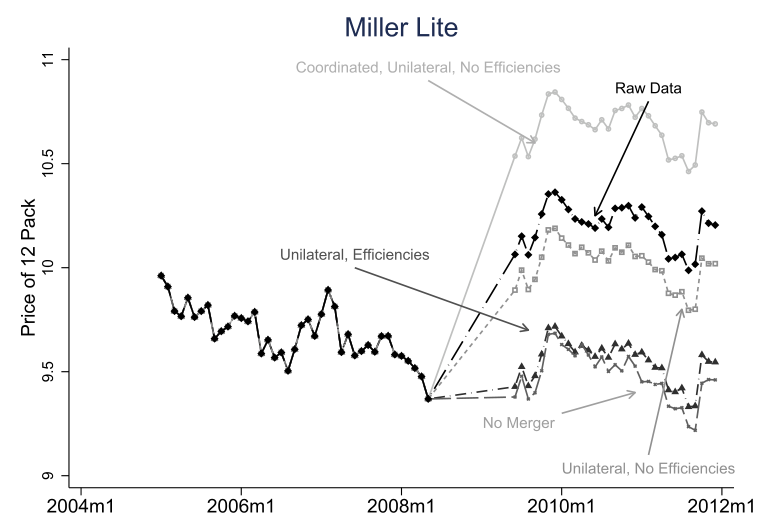
\includegraphics[width=0.82\textwidth]{figures/ch11/mw_fig4_counterfactual.png}
\caption{Counterfactual prices for Miller Lite 12 packs. The series before mid-2008 is the raw data. After the
excluded transition year, the figure shows the raw data and four counterfactual scenarios. They are no merger,
unilateral effects with efficiencies, unilateral effects without efficiencies, and coordinated and unilateral effects
without efficiencies. Each point is the average price across the 39 regions. Source: Miller and Weinberg (2017), Figure 4.}
\label{fig:11-mwcf}
\end{figure}

\begin{table}[htbp]
\centering
\caption{Results from the counterfactual analysis, 2011 (Miller and Weinberg 2017, Table X)}
\label{tab:11-mw-cf}
\footnotesize
\begin{tabular}{@{}lccccc@{}}
\toprule
Coordinated effects & yes & yes & no & no & no \\
Unilateral effects & yes & yes & yes & yes & no \\
Efficiencies & yes & no & yes & no & no \\
 & (i) & (ii) & (iii) & (iv) & (v) \\
\midrule
\multicolumn{6}{@{}l}{\textit{Retail prices (dollars)}} \\
ABI & 10.03 & 10.14 & 9.38 & 9.55 & 9.43 \\
Miller & 8.94 & 9.37 & 8.28 & 8.72 & 8.19 \\
Coors & 10.18 & 10.85 & 9.56 & 10.22 & 9.26 \\
\addlinespace
\multicolumn{6}{@{}l}{\textit{Brewer markups (dollars)}} \\
ABI & 4.45 & 4.56 & 3.81 & 3.97 & 3.84 \\
Miller & 4.52 & 4.32 & 3.83 & 3.63 & 3.05 \\
Coors & 4.25 & 4.06 & 3.61 & 3.41 & 2.68 \\
\addlinespace
\multicolumn{6}{@{}l}{\textit{Welfare statistics (percent change relative to column (v))}} \\
Producer surplus & 22.1 & 19.1 & 10.3 & 8.2 & base \\
\quad ABI & 10.3 & 19.8 & $-0.08$ & 9.3 & base \\
\quad Miller & 37.8 & 20.2 & 24.6 & 9.1 & base \\
\quad Coors & 47.8 & 12.9 & 34.7 & 3.5 & base \\
Consumer surplus & $-3.7$ & $-5.3$ & $-0.2$ & $-2.1$ & base \\
Total surplus & 1.3 & $-0.6$ & 1.8 & $-0.1$ & base \\
\bottomrule
\end{tabular}

\smallskip
\begin{minipage}{0.92\linewidth}
\footnotesize Notes: Prices and markups are volume-weighted means for the 12-pack flagship brands of ABI, Miller and
Coors. Welfare statistics are percent changes relative to the no-merger scenario (v), marked ``base'' (the paper prints a
dash), computed on all products.
Column (i) uses the raw data and the supply estimates, and columns (ii) to (v) are counterfactuals computed with
RCNL-1. All statistics are for 2011. Source: \citet[Table X, p.~1788]{MillerWeinberg2017}.
\end{minipage}
\end{table}

\begin{figure}[htbp]
\centering
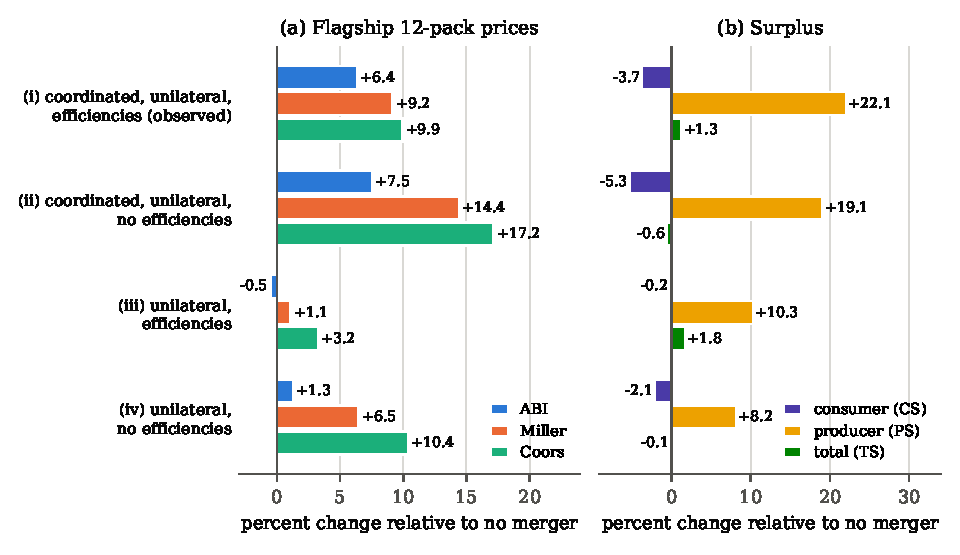
\includegraphics[width=\textwidth]{figures/ch11/mw_counterfactuals.pdf}
\caption{The counterfactual analysis of \cref{tab:11-mw-cf} relative to no merger. Panel (a) shows the percent change
in the volume-weighted price of each brewer's flagship 12 packs, computed from the table's prices. Panel (b) shows the
percent changes in consumer (CS), producer (PS) and total (TS) surplus reported in the table. Our computations from
Miller and Weinberg (2017), Table X.}
\label{fig:11-mwdecomp}
\end{figure}

Prices under no merger lie well below the raw data and roughly continue the pre-merger trend
(\cref{fig:11-mwcf}). The comparisons between columns isolate each channel. All differences below are our
calculations from \cref{tab:11-mw-cf}.

Unilateral effects are large. Moving from column (v) to column (iv) raises the Coors flagship price by \$0.96
(10.4 percent) and the Miller price by \$0.53 (6.5 percent). ABI's price rises by only \$0.12 (1.3 percent), through
strategic complementarity. Consumer surplus falls by 2.1 percent.

Efficiencies are also large, and they roughly offset the unilateral effects. Moving from column (iv) to column
(iii) lowers the Coors price by \$0.66 and the Miller price by \$0.44. ABI's price falls by \$0.17, to slightly below
its no-merger level. With unilateral effects and efficiencies, consumer surplus is only 0.2 percent below the
no-merger level and total surplus is 1.8 percent above it. This is the outcome the DOJ expected when it cleared the
joint venture. The prices of \cref{tab:11-mw-cf} also reveal the size of the efficiency. Price minus markup is ABI's
implied marginal cost, which stays at \$5.57 to \$5.59 in every column. Miller's implied cost is \$5.05 to \$5.14
without efficiencies and \$4.42 to \$4.45 with them. Comparing scenarios that differ only in efficiencies, (ii) with
(i) and (iv) with (iii), Miller's implied cost falls by \$0.63 and \$0.64. Both are close to $\hat\gamma_1 = -0.654$ in
RCNL-1.

Coordination adds a roughly uniform increment to the prices of all three brewers. Comparing column (i) with column (iii), and
column (ii) with column (iv), coordination raises the flagship price by \$0.59 to \$0.66 for each brewer, with and
without efficiencies. Relative to no merger, the observed prices are 6.4 percent higher for ABI, 9.2 percent for
Miller and 9.9 percent for Coors. Consumer surplus is 3.7 percent lower, so coordination accounts for about 3.5
percentage points of the consumer loss. Without efficiencies the loss would have been 5.3 percent.

Coordination is what makes the merger profitable for ABI. With unilateral effects and efficiencies alone, ABI's
producer surplus falls by 0.08 percent, because a more efficient MillerCoors takes sales from it. With coordination
it rises by 10.3 percent. The merging parties gain in every scenario, by 24.6 to 47.8 percent with efficiencies.

The welfare verdict depends on the standard. With coordination, total surplus is still 1.3 percent above the
no-merger level, so ``the antitrust clearance of the merger could be justified under a total welfare standard''
\citep[p.~1788]{MillerWeinberg2017}. Under a consumer surplus standard the merger harmed buyers. The four columns
also reveal the size of consumer surplus relative to total surplus. Solving $TS\% = w\,CS\% + (1-w)\,PS\%$ for the
weight $w$ gives 0.81 in every column, so consumer surplus is about 81 percent of total surplus in the no-merger
benchmark. A 1 percent loss to consumers therefore weighs about four times as much as a 1 percent gain to brewers.

\subsection{Robustness}\label{sec:11-mc-robust}

The paper's main robustness evidence is the spread across the five demand specifications. The estimate of $\kappa$
stays between 0.249 and 0.374 across nested logit and RCNL demand, monthly and quarterly data, and different sets of
income interactions (\cref{tab:11-mw-supply}). The cost coefficients are similarly stable. Four further checks bear on
the main threats.
\begin{enumerate}[label=(\alph*)]
\item A supplemental appendix adds a retail sector. Retail market power changes the
level of brewers' marginal costs but leaves brewer markups largely unaffected \citep[n.~14]{MillerWeinberg2017}.
\item An increasing marginal cost at ABI would bias $\hat\kappa$ upward. The paper
finds little evidence that ABI faced capacity constraints over the sample period \citep[n.~13]{MillerWeinberg2017}.
\item Two specifications ask whether the Great Recession, rather than the merger, triggered softer competition
\citep[Section~5.4]{MillerWeinberg2017}. With a separate $\kappa$ for each post-merger month, the estimates rise over
time as the economy recovers (their Figure~3). The second specification lets $\kappa$ vary with demeaned regional mean
income $\bar D_{rt}$ (unrelated to the aggregate diversion $\bar D$ of \cref{def:11-aggdiv}),
\begin{equation*}
  \kappa_{rt} = \frac{\exp(a_P\,\text{Post}_t + a_D\,\bar D_{rt})}{1 + \exp(a_P\,\text{Post}_t + a_D\,\bar D_{rt})} .
\end{equation*}
Here $a_P$ and $a_D$ are scalar parameters (the paper's $a$ and $b$). Under RCNL-3, $\hat a_P = 0.456$ (0.088) and
$\hat a_D = 0.033$ (0.039), which does not support countercyclical coordination. Under RCNL-1 the estimates are
noisier, $\hat a_P = 0.475$ (0.641) and $\hat a_D = -0.198$ (1.024) (pp.~1785--1786). The authors conclude: ``Given the totality of the evidence, we view the merger as the most likely
catalyst of softer price competition'' (p.~1786).
\item The paper's conclusion states that the price increases of MillerCoors and ABI,
``in both absolute terms and relative to their competitors,'' are ``visually evident and confirmed with econometric
analysis'' \citep[p.~1788]{MillerWeinberg2017}. The econometric analysis regresses the log real retail price on
post-merger indicators for MillerCoors products, for ABI products and for all products \citep[eq.~(1)]{MillerWeinberg2017}.
The regression includes product-by-region fixed effects and a linear time trend. The fullest specification adds
product-specific trends and regional employment and earnings and drops the year after the merger (Table II, column (iv)).
Its MillerCoors and ABI coefficients, which measure price changes relative to the imports, are 0.069 and 0.062, each
with a standard error of 0.007. The descriptive regressions also support the power of the supply instrument
(p.~1780).
\end{enumerate}

\subsection{Assessment}\label{sec:11-mc-assessment}

The paper's central finding is robust within its framework. Given the estimated demand system and the assumption of
parallel cost trends, ABI's post-merger prices are too high for Nash pricing. Whether the finding means that the
merger caused tacit coordination depends on several assumptions, which the literature and the paper itself discuss.

\casehead{What $\kappa$ measures}
By \cref{rem:11-mc-theta}, $\kappa$ is a conduct parameter, and the critique of \citet{Corts1999} applies. Suppose firms
play a repeated game in which the degree of cooperation varies over time. A single estimated weight then summarizes
average behavior, and it need not measure the true degree of collusion (\cref{ch:conduct}). The paper acknowledges the
point and notes that a nonzero $\kappa$ still rejects post-merger Nash pricing \citep[n.~12]{MillerWeinberg2017}. The
same footnote cites \citet{Bresnahan1989} and \citet{Porter1983} on identification with regime shifts. A related
concern is that $\kappa$ is not a structural primitive. Repeated-game theory (\cref{ch:collusion-theory}) predicts
that the sustainable degree of cooperation depends on costs, asymmetries and the number of firms. Scenario (ii)
removes the efficiencies but holds $\kappa$ at $\hat\kappa$. The efficiencies changed MillerCoors's costs and
margins, and with them the gains from cooperation and from deviation. The data do not reveal the value of $\kappa$
without efficiencies, so scenario (ii) is best read as a partial counterfactual.

\casehead{Price leadership}
The internalization weight summarizes outcomes. It leaves open the mechanism that produces them. Documents from the
DOJ's review pointed to leader-follower pricing, and the paper discusses qualitative evidence of price leadership that
surfaced in other beer litigation \citep[pp.~241--242]{AskerNocke2021}. In follow-on work, \citet{MillerSheuWeinberg2021}
investigate this price-leadership mechanism \citep[p.~242, n.~166]{AskerNocke2021}. In their model the leader, ABI, announces supermarkups over
Bertrand prices, and a coalition of ABI, Miller and Coors (later MillerCoors) adopts them
\citep[pp.~3124 and 3140]{MillerSheuWeinberg2021}. Their model gives a mechanism for the coordinated effects that the conduct parameter detects. It also connects this
case to the evidence on price leadership and tacit coordination in \cref{ch:collusion-evidence}.

\casehead{Confounds at the time of the merger}
The identifying assumption is parallel trends in unobserved marginal costs between ABI and the importers
(\cref{prop:11-mc-did}). Several events in the excluded window could violate it. InBev took control of Anheuser-Busch
in November 2008 \citep[p.~1784]{MillerWeinberg2017}, which could have changed ABI's costs or its pricing policy
independently of the joint venture. A change in ABI's objectives that raised its prices would load onto $\hat\kappa$.
The paper notes that the price increases of its Figure 1 predate the close of that deal (n.~16). Exchange rates moved
sharply in late 2008. The monthly average rate rose from 10.1 pesos per dollar in August 2008 to 13.4 in December
\citep{FederalReserve2026}. Corona is shipped from Mexico \citep[n.~4]{MillerWeinberg2017}, so import costs measured
in dollars need not have followed ABI's domestic costs. If import
costs fell relative to ABI's, the model reads ABI's relative price rise as a markup and $\hat\kappa$ is biased upward.
The recession is a further confound. The income interactions and the period effects absorb part of it, and the
domestic sales decline argues against pure down-market substitution. A recession that changed the relative demand for
domestic and imported beer in ways the income interactions miss would still bias the estimate.

\casehead{Retailers and the three-tier system}
The model treats brewers as setting retail prices. In practice brewers set prices to distributors, who set prices to
retailers. Hypothesis (H3), equal retail prices for the three flagship light beers, is a retail convention. The
structural model can only attribute such a pattern to brewer conduct. The retail appendix shows that brewer markups
are robust to retail market power, which addresses the level of costs but not retail pricing conventions.

\casehead{The Nash restriction on imports}
The supply model forces Modelo and Heineken to price as Nash players. The paper motivates this with qualitative
evidence \citep[pp.~1773 and 1779]{MillerWeinberg2017}. The DOJ's complaint against ABI's acquisition of Modelo
alleges that Modelo declined to match many of the price increases led by ABI.
Modelo instead followed a ``Momentum Plan'' designed to grow its share by shrinking its price gaps with domestic premium brands. The complaint does not address Heineken's pricing, and the
paper notes that Heineken's retail prices are similar to Corona's (p.~1773). Anheuser-Busch's equity stake in Modelo, mentioned in \cref{sec:11-mc-industry}, would by itself justify a positive
weight between ABI and Modelo in the sense of \citet{OBrienSalop2000}. Since the importers are the control group in
\cref{prop:11-mc-did}, any softening of their own conduct after the merger would change the comparison.

\casehead{Dependence on substitution patterns}
The estimate of $\kappa$ is the part of ABI's price rise that unilateral effects cannot explain, so it inherits every
restriction of the demand model. \Cref{tab:11-mw-elast} shows substitution close to proportional to shares, with no
special closeness among the domestic light beers. If Bud Light, Miller Lite and Coors Light were closer substitutes
than the RCNL implies, the Nash model would predict a larger response of ABI to MillerCoors's price increase. Less of
the rise would then be left for $\kappa$. A model with a light-beer or domestic nest, or with unobserved random
coefficients, would test this. The nested logit column is consistent with this direction. Its weaker
substitution among inside goods comes with the largest estimate, $\hat\kappa = 0.374$.

\casehead{Measuring efficiencies}
The MillerCoors post-merger indicator absorbs any change in MillerCoors's implied costs relative to the importers.
It therefore measures efficiencies as a residual, and anything else that lowered MillerCoors's implied costs would
be counted as an efficiency. Independent evidence comes from \citet{AshenfelterHoskenWeinberg2015}. They correlate
post-merger price changes across regions with the predicted change in concentration and the predicted reduction in
shipping distances. Larger increases in concentration went with larger price increases, and larger reductions in
shipping distance went with smaller ones \citep[p.~220]{AskerNocke2021}. The timing also differed. Market-power
effects arrived faster than the efficiencies, and cost reductions were ``not fully incorporated into pricing until
about two years after the merger's approval'' (p.~220). A residual measured soon after the merger may therefore
understate the long-run efficiency. The study gives direct evidence that the efficiencies were real. Whether they
were specific to the merger is less clear, as \cref{sec:11-agencies} discusses.

\casehead{Contribution}
\citet{MillerWeinberg2017} changed the empirical analysis of mergers in three ways. First, they showed how to test the
conduct assumption that every merger simulation maintains. They nested Nash pricing in a model with a post-merger
internalization weight and identified the weight from a consummated merger, with non-merging rivals as controls. Second, they
decomposed observed post-merger prices into unilateral effects, coordinated effects and efficiencies, and showed
that the decomposition reverses the welfare verdict between total and consumer surplus standards. Third, they provided
structural evidence for the agencies' concern that a merger can soften competition between the merged firm and its
rivals. The authors call this evidence ``somewhat novel in the empirical literature.'' That literature ``has focused
much more on understanding how mergers affect the unilateral pricing incentives of firms, holding the equilibrium
concept fixed'' \citep[p.~1788]{MillerWeinberg2017}. The case complements the validation exercise of \cref{sec:11-bv}. There a
unilateral-effects simulation underpredicted the observed price increase of the merging firms' rivals, and here a
structural model attributes a similar rival response to coordination.
